\BourbakiFrontMatter{To the Reader}

NEW EDITION

\begin{enumerate}
\def\labelenumi{\arabic{enumi}.}
\item
  The Elements of Mathematics series takes up mathematics at the beginning and gives complete proofs. So in principle, it requires no particular knowledge of mathematics on the readers' part, only a certain familiarity with mathematical reasoning and a certain capacity for abstract thinking. Nevertheless, it is directed primarily at those with a good knowledge of at least the content of the first year or two of university mathematics studies.
\item
  The chosen method of exposition is axiomatic and proceeds typically from the general to the specific. The requirements of proof impose a rigorously fixed order on the subject matter. It follows that the usefulness of certain considerations may not become apparent to readers until later chapters, unless they already have a fairly extended knowledge of mathematics.
\item
  The series is divided into Books and each Book into chapters. The Books that have already been published, either entirely or in part, in the French edition, are listed below. When an English translation is available, the corresponding English title is mentioned between parentheses. Throughout the volume, a reference indicates the English edition when available and the French edition otherwise.
\end{enumerate}

Théorie des ensembles (Theory of Sets) Ref. E (Set Theory)

Algèbre (Algebra \(^{(1)}\) ) --- A (Alg.)

Topologie générale (General Topology) --- TG (Gen.~Top.)

Fonctions d'une variable réelle

(Functions in One Real Variable) --- FVR (FRV)

Espaces vectoriels topologiques

(Topological Vector Spaces)

---

EVT

(Top. Vect. Sp.)

Intégration (Integration)

---

INT

(Int.)

Algèbre commutative

\((Commutative\ Algebra^{(2)})\)

---

AC

(Comm. Alg.)

Variétés différentiables et analytiques

---

VAR

Groupes et algèbres de Lie

(Lie Groups and Lie Algebras)

---

LIE

(Lie)

Théories spectrales

---

TS

Topologie Algébrique

---

TA

In the first six Books (in the order mentioned above), every statement in the text assumes known only the definitions and results already discussed in the same chapters or in the previous chapters in the following order: Set Theory; Alg., Chapters I through III; Gen.~Top., Chapters I through III; Alg./A, from Chapter IV on; Gen.~Top., from Chapter IV on; FRV; Top. Vect. Sp.; Int. From the seventh Book on, the reader will find, if necessary, at the beginning of each Book or chapter, a precise indication of the other Books or chapters used (the first six Books are always assumed known).

\begin{enumerate}
\def\labelenumi{\arabic{enumi}.}
\setcounter{enumi}{3}
\item
  However, certain passages do not follow the rules set out above. They are placed between two asterisks: \(*\ldots\) . In some cases, this is done only to help readers understand the text by including examples that refer to results they may know from other sources. In other cases, we use not only results assumed known in the chapters in question but also results proved elsewhere in the series. These passages are used freely in the parts that assume known the chapters containing them and the chapters they refer to. We hope that the reader will be able to verify the absence of any vicious circle.
\item
  Some Books (either published or in preparation) may include summaries of results. These summaries contain the essential definitions and results of the Book, without any proofs.
\item
  The logical framework of each chapter consists of the chapter's definitions, axioms, and theorems. These are the main parts to keep in mind for subsequent use. Less important results, and those that can be easily recovered from the theorems, are labeled as ``propositions,'' ``lemmas,'' ``corollaries,'' ``remarks,'' etc. Those that may be skipped at first reading are printed in a small font. A commentary on a fundamental theorem occasionally appears under the name of ``scholium.''
\end{enumerate}

To avoid tedious repetitions, it is sometimes convenient to introduce notation or abbreviations that are in force only within a specific chapter or section or subsection of a chapter (for example, in a chapter where all rings are commutative, the word ``ring'' may always refer to a ``commutative ring''). Such conventions are mentioned explicitly at the beginning of the chapter, section, or subsection in which they apply.

Take note that, as in previous chapters of the present Book, fields are not assumed to be commutative unless stated otherwise.

\begin{enumerate}
\def\labelenumi{\arabic{enumi}.}
\setcounter{enumi}{6}
\item
  Some passages are designed to forewarn the reader against serious errors. These passages are indicated in the margin with the sign Z (``dangerous bend'').
\item
  The exercises are meant, on the one hand, to allow readers to verify that they have digested the text well and, on the other hand, to let them acquaint themselves with results that have no place in the text. The most difficult exercises are marked with a ¶.
\item
  We have paid particular attention to the terminology used in this series. We have adhered to the commonly accepted terminology except where there appeared to be good reasons to deviate from it.
\item
  We have made a particular effort to always use rigorously correct language, without sacrificing simplicity. As far as possible, we have drawn attention in the text to any abuses of language or notation, without which any mathematical text runs the risk of becoming pedant, not to say unreadable.
\item
  Since the text consists of the dogmatic exposition of a theory, it rarely contains any references to the literature. Bibliographical references are sometimes gathered together in Historical Notes. The bibliography that follows these Notes contains, in general, only those books and original memoirs that were of the greatest importance in the evolution of the theory under discussion. It does not pretend to be complete.
\end{enumerate}

As to the exercises, we have not deemed it useful to indicate their origin since they have been taken from many different sources (original papers, textbooks, collections of exercises).

\begin{enumerate}
\def\labelenumi{\arabic{enumi}.}
\setcounter{enumi}{11}
\tightlist
\item
  In this chapter of this Book of the new edition, references to theorems, axioms, definitions, remarks, etc. are given by indicating, successively, the Book (using the abbreviation listed in No.~3), chapter, section, subsection, and page where they can be found. The reference to the Book is left out when it is the same as the present Book. For example, in the Book Algebra,
\end{enumerate}

\textbf{Set Theory, III, § 4, No.~2, p.~167, Corollary 3}

refers to Corollary 3 of § 4, No.~2 on page 167 of Chapter III of the Book Set Theory;

\textbf{II, § 1, No.~11, p.~215, Proposition 17}

refers to Proposition 17 of § 1, No.~11 on page 215 of Chapter II of the Book Algebra.

The summaries of results are indicated by the letter R; for example, Top. Vect. Sp., R refers to the ``summary of results'' of the Book Topological Vector Spaces.

As some Books will be published later in the new edition, references to those Books consist of, successively, the Book, chapter, section, and subsection where the results in question should be, for example,

\textbf{Comm. Alg., III, § 4, No.~5, Corollary of Proposition 6.}

When a reference to a volume of the French edition is made, the acronyms in upright capitals are used, and the French terminology and typography is used; for example,

\textbf{TA, II, § 2, n° 4, p.~158, corollaire de la proposition 1}

refers to the corollary of Proposition 1 of § 2, No.~4 on page 158 of Chapter II of the Book Topologie Algébrique.

\BourbakiFrontMatter{Introduction}

This chapter is devoted to the study of certain classes of rings and that of modules over these rings. There are several underlying themes behind this study, such as classification or decomposition questions or the description of subobjects and of sets of morphisms.

We essentially only deal with these questions under reasonable finiteness assumptions, which is why the chapter opens with the notions of module and of Noetherian and Artinian rings.

As far as rings are concerned, we present several results that allow one to understand Artinian rings:

\begin{enumerate}
\def\labelenumi{\alph{enumi})}
\item
  The Jacobson radical of an Artinian ring is its nilradical ( \(\S10\) ), and the corresponding quotient is a semisimple ring ( \(\S8\) ).
\item
  A semisimple ring is isomorphic to the product of a finite family of simple rings (§7).
\item
  By Wedderburn's theorem (VIII, p.~120, Theorem 1), a simple ring is isomorphic to a matrix algebra over a field.
\end{enumerate}

Up to Morita equivalence ( \(\S6\) ), an algebra of finite degree that is a simple ring is determined by its class in an abelian group called the Brauer group. We give several descriptions of this group ( \(\S15\) and \(\S16\) ), as well as examples ( \(\S18\) and \(\S19\) ).

For modules, we present two natural decompositions: The first, in terms of composition series (I, §4, No.~7, p.~41, Definition 9), is provided by the Jordan--Hölder theorem (I, §4, No.~7, p.~43, Theorem 6). The second, which corresponds to direct sums, is given in the case of modules of finite length by the Krull--Remak--Schmidt theorem (VIII, p.~37, Theorem 2), which, here, we deduce from a result of Azumaya on semiprimordial modules (VIII, p.~32,

Theorem 1). We also consider the invariants associated with modules that behave additively for the decompositions mentioned above; the Grothendieck groups described in §11 are solutions of universal problems for these invariants. When we study the structure of modules over a ring, the notion of ring isomorphism is, to our advantage replaced by Morita equivalence.

For semisimple modules, that is, direct sums of simple modules, the notion of description of a module (VIII, p.~69, Definition 5) allows us to describe the homomorphisms arising from the module as well as its submodules.

By way of illustration, in §21, we consider the case of the algebra of a finite group, whose modules correspond to the linear representations of the group.

A historical note included at the end of the volume, copied from the previous edition, retraces how many of the notions developed here arose.

\BourbakiMainMatter
\setcounter{chapter}{7}
\chapter{Semisimple Modules and Rings}

In this chapter, when we speak of a module (without further specification), we mean a left module. Let A be a ring and M an A-module. For any \(a \in A\) , we denote the homothety \(x \mapsto ax\) of M by \(a_{M}\) . The mapping \(a \mapsto a_{M}\) is a homomorphism from the ring A to a subring \(A_{M}\) of \(\operatorname{End}_{\mathbf{Z}}(\mathrm{M})\) , which we call the ring of homotheties of M.

Unless stated otherwise, the algebras we consider are associative and unital; by a subalgebra of an algebra E, we mean a subalgebra containing the unit element of E; the algebra homomorphisms are assumed to be unital.

Let K be a commutative ring and L a commutative K-algebra. For any K-module E, we denote the L-module \(L \otimes_{K} E\) derived from it by extension of scalars by \(\mathrm{E}_{(\mathrm{L})}\) (II, §5, No.~1, p.~277). If A is a K-algebra and M a left A-module, then \(\mathrm{A}_{(\mathrm{L})}\) is endowed with a natural L-algebra structure (III, §1, No.~5, p.~433) and \(\mathrm{M}_{(\mathrm{L})}\) is endowed with the left \(\mathrm{A}_{(\mathrm{L})}\) -module structure with law of action given by the formula \((\lambda \otimes a)(\mu \otimes m) = \lambda \mu \otimes am\) .

For any commutative ring K and any group G, we denote the algebra \(\mathrm{K}^{(\mathrm{G})}\) of G over the ring K by K{[}G{]} (III, §2, No.~6, p.~446).

\section{Artinian Modules and Noetherian Modules}

\subsection{Artinian Modules and Noetherian Modules}

DEFINITION 1. --- Let A be a ring. We call an A-module M Artinian (resp. Noetherian) if it satisfies the following equivalent conditions:

\begin{enumerate}
\def\labelenumi{(\roman{enumi})}
\item
  Every nonempty set of submodules of M, ordered by inclusion, has a minimal (resp. maximal) element.
\item
  Every decreasing (resp. increasing) sequence of submodules of M is stationary.
\end{enumerate}

The equivalence of conditions (i) and (ii) follows from Set Theory, III, §6, No.~5, p.~190, Proposition 6.

An A-module M is Artinian (resp. Noetherian) if and only if M, viewed as a module over the ring of homotheties \(A_{M}\) , is Artinian (resp. Noetherian).

Let M be an Artinian (resp. Noetherian) A-module. Every nonempty set of submodules of M, ordered by inclusion, that is left directed (resp. right directed) has a least element (resp. a greatest element) (Set Theory, III, §1, No.~10, p.~145, Proposition 10).

Let M be an Artinian (resp. Noetherian) A-module and \((\mathrm{M}_{i})_{i\in\mathrm{I}}\) a family of submodules of M. The intersections (resp. sums) of finite subfamilies of the family \((\mathrm{M}_{i})_{i\in\mathrm{I}}\) form a nonempty left (resp. right) directed set of submodules of M. Therefore, there exists a finite subset J of I such that \(\bigcap_{i\in I}M_{i}=\bigcap_{i\in J}M_{i}\) (resp. \(\sum_{i\in I}M_{i}=\sum_{i\in J}M_{i}\) ).

Examples. --- 1) A finite-dimensional vector space over a field is Artinian and Noetherian.

\begin{enumerate}
\def\labelenumi{\arabic{enumi})}
\setcounter{enumi}{1}
\tightlist
\item
  Let M be an A-module. If there exists an infinite family \((\mathrm{M}_{i})_{i\in\mathrm{I}}\) of nonzero submodules of M whose sum is direct, then M is neither Artinian nor Noetherian: indeed, for every strictly decreasing (resp. strictly increasing) infinite sequence \((\mathrm{J}_{n})\) of subsets of I, the infinite sequence \((\sum_{i\in\mathrm{J}_{n}}\mathrm{M}_{i})\) of submodules of M is strictly decreasing (resp. strictly increasing). In particular, an infinite-dimensional vector space over a field is neither Artinian nor Noetherian.
\end{enumerate}

*3) We will see further on that the Z-module Z is Noetherian but not Artinian (VIII, p.~5, Example 3).*

\begin{enumerate}
\def\labelenumi{\arabic{enumi})}
\setcounter{enumi}{3}
\tightlist
\item
  Let \(p\) be a prime number and \(\mathrm{M}_p\) the \(p\) -primary component of the torsion \(\mathbf{Z}\) -module \(\mathbf{Q} / \mathbf{Z}\) (VII, §2, No.~2, p.~7). Every submodule of \(\mathrm{M}_p\) is equal to either \(\mathrm{M}_p\) or \(p^{-n}\mathbf{Z} / \mathbf{Z}\) for an integer \(n \in \mathbf{N}\) (VII, §2, p.~54, Exercise 3). Consequently, \(\mathrm{M}_p\) is an Artinian but not Noetherian \(\mathbf{Z}\) -module.
\end{enumerate}

PROPOSITION 1. --- An A-module M has finite length (II, §1, No.~10, p.~212) if and only if it is both Artinian and Noetherian.

Suppose that M has finite length d.~Then every strictly increasing or strictly decreasing sequence of submodules of M has at most \(d+1\) terms (I, §4, No.~7, p.~44). Consequently, M is Artinian and Noetherian.

Conversely, suppose that M is Artinian and Noetherian. Let S be the set of submodules of M of finite length. The zero submodule is an element of S, and since M is Noetherian, S has a maximal element N. Let us give a proof by contradiction and suppose that \(M \neq N\) . The set of submodules of M distinct from N and containing N then has a minimal element P because M is Artinian. The module P/N has length 1, and since N is a module of finite length, the same holds for P (II, §1, No.~10, p.~212, Proposition 16). This contradicts the definition of N.

PROPOSITION 2. --- An A-module M is Noetherian if and only if every submodule of M is finitely generated.

Begin by assuming that every submodule of M is finitely generated. Let \((\mathrm{P}_{n})_{n\in\mathbf{N}}\) be an increasing sequence of submodules of M, and let P be its union. This is a submodule of M. By assumption, there exists a finite subset F of M generating the module P; let \(n\in N\) be an integer such that \(F\subset P_{n}\) . We then have \(P_{n}=P\) , and the sequence \((\mathrm{P}_{n})_{n\in\mathbf{N}}\) is stationary. This proves that the module M is Noetherian.

The converse is a consequence of the following more precise statement.

Lemma 1. --- Let M be a Noetherian A-module and E a subset of M. There exists a finite subset F of E generating the same submodule as E.

Indeed, by VIII, p.~2, there exists a finite subset F of E such that \(\sum_{x\in E}Ax=\sum_{x\in F}Ax\) .

PROPOSITION 3. --- Let M be an A-module and N a submodule of M. Then M is Artinian (resp. Noetherian) if and only if N and M/N are.

We will give the proof in the case of Artinian modules; the case of Noetherian modules is analogous.

Suppose that M is Artinian. Since every submodule of N is a submodule of M, the module N is Artinian. Let \((\mathrm{P}_{n})_{n\in\mathbf{N}}\) be a decreasing sequence of submodules of M/N. There exists a decreasing sequence \((\mathrm{Q}_{n})_{n\in\mathbf{N}}\) of submodules of M containing N such that \(P_{n}=Q_{n}/N\) for every \(n\in N\) (I, §4, No.~6, p.~41, Theorem 4). Since M is Artinian, the sequence \((\mathrm{Q}_{n})\) is stationary, hence so is the sequence \((\mathrm{P}_{n})\) . Consequently, the module M/N is Artinian.

Conversely, suppose that the modules N and M/N are Artinian, and consider a decreasing sequence \((\mathrm{P}_{n})\) of submodules of M. The sequence \(P_{n}^{\prime} = N \cap P_{n}\) of submodules of N is stationary. Likewise, the sequence \(\mathrm{P}_{n}^{\prime\prime} = (\mathrm{N} + \mathrm{P}_{n})/\mathrm{N}\) of submodules of M/N is stationary. Hence, there exists an integer \(m \in N\) such that we have \(P_{n}^{\prime} = P_{m}^{\prime}\) and \(P_{n}^{\prime\prime} = P_{m}^{\prime\prime}\) for every integer \(n \geqslant m\) . The sequence \((\mathrm{P}_{n})\) is then stationary by the following lemma.

Lemma 2. --- Let M be an A-module and N, P, and Q submodules of M. Suppose that we have \(P \subset Q\) , \(N \cap P = N \cap Q\) , and \(N + P = N + Q\) . We then have P = Q.

Let x be an element of Q. It belongs to \(N + P\) ; hence, there exists an element y of P such that \(x - y \in N\) . Since Q contains P, the difference x - y belongs to \(N \cap Q\) and therefore to P. Consequently, x belongs to P.

COROLLARY. --- Let M be an A-module and \((\mathrm{M}_{i})_{i\in\mathrm{I}}\) a finite family of submodules of M.

\begin{enumerate}
\def\labelenumi{\alph{enumi})}
\item
  If the modules \(\mathrm{M}_i\) are Artinian (resp. Noetherian), then so is their sum \(\sum_{i\in \mathrm{I}}\mathrm{M}_i\) .
\item
  If the modules \(\mathrm{M} / \mathrm{M}_i\) are Artinian (resp. Noetherian), then so is the module \(\mathrm{M} / \bigcap_{i\in \mathrm{I}}\mathrm{M}_i\) .
\end{enumerate}

By induction, it suffices to treat the case when \(I = \{1, 2\}\) . The module \(M_{2}/(M_{1} \cap M_{2})\) , quotient of \(M_{2}\) , is isomorphic to the submodule \((M_{1} + M_{2})/M_{1}\) of \(M/M_{1}\) (I, §4, No.~6, p.~41, Theorem 4).

In part a), we assume that \(\mathrm{M}_1\) and \((\mathrm{M}_1 + \mathrm{M}_2) / \mathrm{M}_1\) are Artinian (resp. Noetherian); the same then holds for \(\mathrm{M}_1 + \mathrm{M}_2\) (Proposition 3).

In part b), we assume that \(M/M_{2}\) and \(M_{2}/(M_{1} \cap M_{2})\) are Artinian (resp. Noetherian); the same then holds for \(M/(M_{1} \cap M_{2})\) (loc. cit.).

Example 5. --- Let \((\mathrm{M}_{i})_{i\in\mathrm{I}}\) be a finite family of A-modules. If the modules \(M_{i}\) are Artinian (resp. Noetherian), then so is their direct sum \(\bigoplus_{i\in I} M_{i}\) .

Remark. --- The definitions and results of this subsection extend to arbitrary abelian groups with operators by replacing the submodules in the statements with stable subgroups.

\subsection{Artinian Rings and Noetherian Rings}

DEFINITION 2. --- A ring A is said to be left Artinian (resp. left Noetherian) if the left A-module \(A_{s}\) is Artinian (resp. Noetherian). Likewise, a ring A is said to be right Artinian (resp. right Noetherian) if the right A-module \(A_{d}\) is Artinian (resp. Noetherian).

A ring A is right Artinian (resp. right Noetherian) if and only if its opposite ring \(A^{o}\) is left Artinian (resp. left Noetherian). For a commutative ring A, the properties of being left Artinian and of being right Artinian coincide, and when they are hold, we say that the ring A is Artinian; we adopt an analogous convention for ``Noetherian.'' There exist noncommutative rings that are left Artinian but not right Artinian, and noncommutative rings that are left Noetherian but not right Noetherian (VIII, p.~14, Exercise 3).

Let \(A\) be a ring. By definition, the following properties are equivalent:

\begin{enumerate}
\def\labelenumi{(\roman{enumi})}
\item
  The ring A is left Artinian.
\item
  Every nonempty set of left ideals of A, ordered by inclusion, has a minimal element.
\item
  Every decreasing sequence of left ideals of A is stationary.
\end{enumerate}

Because of Proposition 2 of VIII, p.~3, the following properties are equivalent:

\begin{enumerate}
\def\labelenumi{(\roman{enumi})}
\item
  The ring A is left Noetherian.
\item
  Every nonempty set of left ideals of A, ordered by inclusion, has a maximal element.
\item
  Every increasing sequence of left ideals of A is stationary.
\item
  Every left ideal of A is generated by a finite subset of A.
\end{enumerate}

Examples. --- 1) A field is a ring that is both left and right Artinian and Noetherian.

\begin{enumerate}
\def\labelenumi{\arabic{enumi})}
\setcounter{enumi}{1}
\item
  Let A be a ring and D a subring of A. Suppose that D is a field and that A is a finite-dimensional left vector space over D. Then the ring A is left Artinian and left Noetherian because every left ideal of A is a D-vector subspace of A. In particular, a finite-dimensional algebra over a commutative field is a ring that is both left and right Artinian and Noetherian.
\item
  A principal ideal domain (VII, §1, No.~1, p.~1, Definition 1) is Noetherian. An integral domain A that is not a field is not an Artinian ring: for every nonzero noninvertible element \(a\) of A, the sequence of ideals \(a^n\mathbf{A}\) (for \(n \in \mathbf{N}\) ) is strictly decreasing. In particular, the ring \(\mathbf{Z}\) of integers is Noetherian but not Artinian.
\item
  Let M be an A-module that is the direct sum of an infinite family \((\mathrm{M}_{i})_{i\in\mathrm{I}}\) of nonzero submodules. Let E be the endomorphism ring of M. For every \(i\in I\) , let \(a_{i}\) (resp. \(b_{i}\) ) be the set of elements of E with kernel containing \(\sum_{j\neq i}M_{j}\) (resp. with image contained in \(M_{i}\) ). Then \((a_{i})\) is an infinite family of nonzero left ideals of E whose sum is direct, and \((b_{i})\) is an infinite family of nonzero right ideals of E whose sum is direct. Consequently, the ring E is neither left nor right Artinian (resp. Noetherian) (VIII, p.~2, Example 2). In particular, the endomorphism ring of an infinite-dimensional vector space is neither left nor right Artinian (resp. Noetherian).
\end{enumerate}

THEOREM 1. --- Let A be a left Artinian ring. The A-module \(A_{s}\) has finite length.

We will use the following lemma in the proof.

Lemma 3. --- Let A be a ring and n a natural number. An Artinian A-module M that is the sum of a family of submodules of length \(\leqslant n\) has finite length.

We use induction on n.~First, suppose n = 1. If M were not of finite length, then we could construct a sequence \((\mathrm{M}_{m})_{m \in \mathbf{N}}\) of submodules of M of length 1 with \(M_{m} \not\subset (\sum_{i < m} M_{i})\) for every \(m \in N\) . We would then have \(M_{m} \cap \sum_{i < m} M_{i} = 0\) for every m, and the sum of the family \((\mathrm{M}_{m})_{m \in \mathbf{N}}\) would be direct. However, this contradicts the fact that the A-module M is Artinian (VIII, p.~2, Example 2).

Now, suppose \(n \geqslant 2\) . Let \((\mathrm{M}_{i})_{i \in \mathrm{I}}\) be a family of submodules of M of length \(\leqslant n\) with sum M. For every \(i \in I\) , choose a submodule \(M_{i}^{\prime}\) of \(M_{i}\) of length \(\leqslant n - 1\) such that \(M_{i}/M_{i}^{\prime}\) has length \(\leqslant 1\) . Set \(M^{\prime} = \sum M_{i}^{\prime}\) , and denote the image of \(M_{i}\) in \(M^{\prime\prime} = M/M^{\prime}\) by \(M_{i}^{\prime\prime}\) . The modules \(M_{i}^{\prime\prime}\) are of length \(\leqslant 1\) , and their sum is \(M^{\prime\prime}\) . The modules \(M^{\prime}\) and \(M^{\prime\prime}\) are Artinian (VIII, p.~3, Proposition 3); by the induction hypothesis, they are of finite length. Hence, M has finite length (II, §1, No.~10, p.~212, Proposition 16).

Let us now prove Theorem 1. Let S denote the set of left ideals a of A such that the module \(A_{s}/a\) has finite length. Let \((\mathfrak{a}_{i})_{i\in I}\) be a finite family of elements of S. By Proposition 1 of VIII, p.~2, the A-module \(A_{s}/a_{i}\) is Artinian and Noetherian for every \(i\in I\) . Consequently, \(A_{s}/\bigcap_{i\in I}a_{i}\) is Artinian and Noetherian (VIII, p.~4, Corollary of Proposition 3), hence of finite length (VIII, p.~2, Proposition 1). This proves that S is a left directed set for the inclusion. Since the ring A is left Artinian, the set S has a least element b. We denote the length of the A-module \(A_{s}/b\) by n.

Let \(x\) be an element of \(A_s\) and \(\mathfrak{a}\) its annihilator (II, §1, No.~12, p.~219). The A-module \(Ax\) is isomorphic to \(A_s / \mathfrak{a}\) . If \(Ax\) has finite length, then \(\mathfrak{a}\) belongs to \(\mathscr{S}\) , so \(\mathfrak{a}\) contains \(\mathfrak{b}\) and \(Ax\) has length \(\leqslant n\) . Thus, every monogenous left ideal of \(A\) of finite length has length \(\leqslant n\) . Let \(\mathfrak{c}\) be the sum of these ideals; this is a left ideal of \(A\) , of finite length by Lemma 3. Every left ideal of \(A\) of finite length is a sum of monogenous left ideals of finite length and is therefore contained in \(\mathfrak{c}\) . Hence, \(\mathfrak{c}\) is the largest left ideal of \(A\) of finite length.

If c were distinct from A, then the set of left ideals of A containing c and distinct from c would have a minimal element \(c'\) . The A-module \(c'/c\) would then have length 1, and \(c'\) would have finite length, which contradicts the fact that c is maximal. We therefore have c = A; the A-module \(A_{s}\) has finite length.

COROLLARY. --- Every left Artinian ring is left Noetherian.

Let \(A\) be a left Artinian ring. By Theorem 1, the \(A\) -module \(A_s\) has finite length. We then apply Proposition 1 of VIII, p.~2.

Let A be a left (resp. right) Artinian ring; the length of the A-module \(A_{s}\) (resp. \(A_{d}\) ) (I, §4, No.~7, p.~44) is called the left (resp. right) length of the ring A. When A is a commutative Artinian ring, these two lengths coincide and are simply called the length of A. When A is left and right Artinian but is not commutative, the left and right lengths of A are not necessarily equal (VIII, p.~14, Exercise 3).

Example 5. --- The left and right lengths of a field are equal to 1.

PROPOSITION 4. --- a) Let A be a left Noetherian ring and M a finitely generated left A-module. The module M is Noetherian, and every submodule of M is finitely generated.

\begin{enumerate}
\def\labelenumi{\alph{enumi})}
\setcounter{enumi}{1}
\tightlist
\item
  Let A be a left Artinian ring and M a left A-module. The following properties are equivalent: the module M is finitely generated; the module M is Artinian; the module M has finite length; the module M is Noetherian.
\end{enumerate}

Let us prove a). Every monogenous submodule of M is isomorphic to a quotient of \(A_{s}\) , hence is Noetherian by Proposition 3 of VIII, p.~3. The module M is a finite sum of such submodules; it is therefore Noetherian by the corollary (VIII, p.~4) of Proposition 3. Every submodule of M is then finitely generated (VIII, p.~3, Proposition 2)

Now, suppose that the ring A is left Artinian. We see, as in the previous section, that if the A-module M is finitely generated, then it is Artinian. If it is Artinian, then it has finite length: indeed, its monogenous submodules are isomorphic to quotients of \(A_{s}\) and are therefore of finite length less than that of \(A_{s}\) , and the assertion follows from Lemma 3. Every module of finite length is Noetherian, and every Noetherian module is finitely generated. This proves b).

PROPOSITION 5. --- a) Let A be a left Artinian (resp. left Noetherian) ring, and let \(\varphi : \mathrm{A} \to \mathrm{B}\) be a ring homomorphism that makes B into a finitely generated left A-module. The ring B is left Artinian (resp. left Noetherian).

\begin{enumerate}
\def\labelenumi{\alph{enumi})}
\setcounter{enumi}{1}
\item
  Let A be a left Artinian (resp. left Noetherian) ring, and let \(\mathfrak{a}\) be a two-sided ideal of A; the ring A/ \(\mathfrak{a}\) is left Artinian (resp. left Noetherian).
\item
  Let \((\mathrm{A}_i)_{i\in \mathrm{I}}\) be a family of left Artinian (resp. left Noetherian) rings. The ring \(\prod_{i\in \mathrm{I}}\mathrm{A}_i\) is left Artinian (resp. left Noetherian).
\end{enumerate}

We will treat the case of Artinian rings; the case of Noetherian rings is analogous.

Let us prove a). By Proposition 4, the ring \(\mathrm{B}_s\) is an Artinian left A-module and a fortiori an Artinian left B-module.

Assertion b) follows from assertion a) applied to the canonical homomorphism from A to A/a.

Let us prove c). Set \(A = \prod_{i \in I} A_i\) . By assumption, \((\mathrm{A}_i)_s\) is an Artinian left \(A_i\) -module and a fortiori an Artinian left A-module. By Example 5 of VIII, p.~4, the A-module \(A_s\) is Artinian.

COROLLARY. --- The prime ideals of an Artinian commutative ring are its maximal ideals.

In any commutative ring, a maximal ideal is prime. Let A be an Artinian commutative ring. Let p be a prime ideal of A. The ring A/p is an integral domain and is Artinian (Proposition 5), hence is a field (VIII, p.~5, Example 3). Consequently, the ideal p is maximal.

\pandocbounded{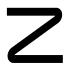
\includegraphics[keepaspectratio]{images/part001_e30b1f1b.jpg}}

The polynomial ring \(\mathbf{Q}[(\mathrm{X}_{n})_{n\in\mathbf{N}}]\) is an integral domain; it is not Noetherian (or Artinian) (VIII, p.~15, Exercise 9). It is a subring of its field of fractions, which is an Artinian (and Noetherian) ring.

\subsection{Countermodule}

DEFINITION 3. --- Let A be a ring, M an A-module, and \(E = \text{End}_{A}(M)\) the endomorphism ring of M. The countermodule of M is the left E-module with the same underlying additive group as M and external law \((c, x) \mapsto c(x)\) .

Let Z be the center of the ring A. For every \(a \in Z\) , the homothety \(a_{M}\) belongs to E. Consequently, E is canonically endowed with the structure of a Z-algebra. In particular, if M is a finitely generated Z-module, then the countermodule of M is finitely generated.

Lemma 4. --- Let M be a left A-module with finitely generated countermodule. There exist a natural number m and an injective \(A_{M}\) -linear mapping from \((\mathrm{A}_{\mathrm{M}})_{s}\) to \(M^{m}\) .

Set \(\mathrm{E}=\mathrm{End}_{\mathrm{A}}(\mathrm{M})\) . Let \((x_{1},\ldots,x_{m})\) be a finite generating family of the E-module M. The mapping \(\varphi:a\mapsto(ax_{1},\ldots,ax_{m})\) from \((\mathrm{A}_{\mathrm{M}})_{s}\) to \(M^{m}\) is \(A_{M}\) -linear. Let a be an element of \(A_{M}\) such that \(\varphi(a)=0\) . The set of elements x of M such that ax = 0 is an E-submodule of M containing \(x_{1}, \ldots, x_{m}\) and is therefore equal to M, which implies a = 0.

PROPOSITION 6. --- Let M be an Artinian (resp. Noetherian) left A-module with finitely generated countermodule. The ring of homotheties \(A_{M}\) of M is left Artinian (resp. left Noetherian).

This follows from Lemma 4 and Proposition 3 of VIII, p.~3.

COROLLARY. --- Let A be a commutative ring.

\begin{enumerate}
\def\labelenumi{\alph{enumi})}
\item
  Let M be a Noetherian A-module. The ring \(A_{M}\) is Noetherian.
\item
  Let M be an A-module of finite length. The ring \(A_{M}\) is Artinian.
\end{enumerate}

Let M be an A-module. Under the assumptions of a) or b), the A-module M is finitely generated. Since A is commutative, \(A_{M}\) is contained in the ring \(\operatorname{End}_{\mathrm{A}}(\mathrm{M})\) , so that the countermodule of M is finitely generated. It then suffices to apply Proposition 6.

Remark. --- Let A be a ring. An Artinian left A-module M with finitely generated countermodule has finite length: indeed, the ring of homotheties \(A_{M}\) of M is left Artinian (Proposition 6), and M is an Artinian module over \(A_{M}\) ; by VIII, p.~7, Proposition 4, the module M has finite length over \(A_{M}\) and therefore also over A.

In particular, every finitely generated Artinian module over a commutative ring has finite length. By contrast, a finitely generated Artinian module over a noncommutative ring is not necessarily of finite length (VIII, p.~16, Exercise 12).

\subsection{Polynomials with Coefficients in a Noetherian Ring}

Let A be a ring, \(\sigma\) an endomorphism of the ring A, and d an endomorphism of the additive group of A satisfying the relation

\[
d (a b) = \sigma (a) d (b) + d (a) b\tag{1}
\]

for all \(a, b \in A\) . In other words, d is a derivation from the ring A to the (A,A)-bimodule obtained by endowing the additive group of A with the left law of action \((a, x) \mapsto \sigma(a)x\) and the right law of action \((x, a) \mapsto xa\) . We have \(d(1) = 0\) (III, §10, No.~5, p.~557, Proposition 3).

Recall (IV, §1, No.~1, p.~2) that A{[}X{]} denotes the Z-module \(A \otimes_{Z} Z[X]\) of polynomials in one variable with coefficients in A. We endow it with its natural structure of a left A-module. The family \((\mathrm{X}^{n})_{n \in \mathbf{N}}\) is a basis for A{[}X{]} over A. We identify A with its image under the mapping \(a \mapsto a \otimes 1\) .

PROPOSITION 7. --- Let A, \(\sigma\) , \(d\) be as above. There exists a unique ring structure on the group A{[}X{]} with the following properties:

\begin{enumerate}
\def\labelenumi{\alph{enumi})}
\item
  The addition in this ring is the usual addition of A{[}X{]}.
\item
  The multiplication in this ring extends that of A.
\item
  The product in this ring of a sequence \((a,X,\ldots,X)\) , consisting of an element a of A followed by n terms equal to X, is the polynomial \(aX^{n}\) .
\item
  In this ring, we have \(\mathrm{X}a = \sigma(a)\mathrm{X} + d(a)\) for every \(a \in \mathrm{A}\) .
\end{enumerate}

Let E be the endomorphism ring of the additive group A{[}X{]}. The mapping that sends \(a \in A\) to the homothety \(a_{M}\) of the left A-module M = A{[}X{]} is a ring homomorphism from A to E. Consider the elements u, \(\sigma_{M}\) , and \(d_{M}\) of E defined by \(u(\sum b_{n}X^{n}) = \sum b_{n}X^{n+1}\) , \(\sigma_{\mathrm{M}}(\sum b_{n}X^{n}) = \sum \sigma(b_{n})X^{n}\) , \(d_{\mathrm{M}}(\sum b_{n}X^{n}) = \sum d(b_{n})X^{n}\) . For every \(a \in A\) , we have

\[
u a _ {\mathrm{M}} = a _ {\mathrm{M}} u, \quad \sigma_ {\mathrm{M}} a _ {\mathrm{M}} = \sigma (a) _ {\mathrm{M}} \sigma_ {\mathrm{M}}, \quad d _ {\mathrm{M}} a _ {\mathrm{M}} = \sigma (a) _ {\mathrm{M}} d _ {\mathrm{M}} + (d (a) _ {\mathrm{M}}).\tag{2}
\]

\[
X_ {M} = \sigma_ {M} u+ d_ {M} .\tag{3}
\]

It follows from (2) that for every \(a \in \mathbf{A}\) , we have

\[
\mathrm{X} _ {\mathrm{M}} a _ {\mathrm{M}} = \sigma (a) _ {\mathrm{M}} \mathrm{X} _ {\mathrm{M}} + (d (a) _ {\mathrm{M}}).\tag{4}
\]

Consider the mapping \(\varphi : \mathrm{A}[\mathrm{X}] \to \mathrm{E}\) defined by

\[
\varphi \Bigl (\sum a _ {n} \mathrm{X} ^ {n} \Bigr) = \sum (a _ {n}) _ {\mathrm{M}} (\mathrm{X} _ {\mathrm{M}}) ^ {n}.\tag{5}
\]

This is a group homomorphism. An induction argument shows that we have \((\mathrm{X}_{\mathrm{M}})^{n}(1)=\mathrm{X}^{n}\) for every \(n\in N\) . We therefore have \(\varphi(\mathrm{P})(1)=\mathrm{P}\) for every \(P\in\mathrm{A}[X]\) , which proves that the homomorphism \(\varphi\) is injective. We denote its image by B. The set B is a subgroup of E; it contains 1, and it is stable under left multiplication by \(a_{M}\) for \(a\in A\) and by \(X_{M}\) (see (4)). It is therefore a subring of E. The unique ring structure on A{[}X{]} derived from that on B by transfer of structure via \(\varphi\) has the properties of Proposition 7, where property d) results from relation (4).

If A{[}X{]} is endowed with a ring structure that has the properties of Proposition 7, then the left homothety \(\gamma_{X}\) of this ring (I, §8, No.~1, p.~97) necessarily sends \(bX^{n}\) to \(\sigma(b)\mathrm{X}^{n+1} + d(b)\mathrm{X}^{n}\) for \(b \in A\) and \(n \in N\) , hence is equal to \(X_{M}\) . The homothety \(\gamma_{a}\) is necessarily equal to \(a_{M}\) for every \(a \in A\) . Consequently, we have \(\gamma_{\mathrm{P}} = \varphi(\mathrm{P})\) for every \(P \in A[X]\) ; the uniqueness in Proposition 7 follows.

The set A{[}X{]}, endowed with the unique ring structure with the properties of Proposition 7, is denoted by \(A[X]_{\sigma,d}\) and called the polynomial ring in X with coefficients in A, relative to \(\sigma\) and d.~We simply denote it by \(A[X]_{\sigma}\) when d is the zero mapping and by A{[}X{]} when, moreover, \(\sigma\) is the identity mapping on A. This notation is compatible with that introduced in IV, §1, No.~1, p.~1 for a commutative ring A.

Remark. --- The ring \(A[X]_{\sigma,d}\) has the following universal property: given a ring \(A'\) , a ring homomorphism \(f: A \to A'\) , and an element x of \(A'\) such that \(xf(a) = f(\sigma(a))x + f(d(a))\) for every \(a \in A\) , there exists a unique ring homomorphism \(g: A[X]_{\sigma,d} \to A'\) that extends f and maps X onto x.

The uniqueness is clear. Let us therefore show that the mapping \(g: \mathrm{A}[\mathrm{X}]_{\sigma,d} \to \mathrm{A}'\) defined by \(g(\sum a_n\mathrm{X}^n) = \sum f(a_n)x^n\) has the required properties. It extends \(f\) , maps \(\mathrm{X}\) onto \(x\) , and is a group homomorphism. We have \(g(1) = 1\) . For \(a \in \mathrm{A}\) and \(\mathrm{Q} = \sum a_n\mathrm{X}^n\) in \(\mathrm{A}[\mathrm{X}]_{\sigma,d}\) , we have

\[
g (a \mathrm{Q}) = g \left(\sum a a _ {n} X ^ {n}\right) = \sum f (a a _ {n}) x ^ {n} = f (a) \sum f (a _ {n}) x ^ {n} = g (a) g (\mathrm{Q})
\]

as well as

\[
\begin{array}{l} g (\mathrm{XQ}) = g \Bigl (\sum \Bigl (\sigma (a _ {n}) \mathrm{X} ^ {n + 1} + d (a _ {n}) \mathrm{X} ^ {n} \Bigr) \Bigr) \\ = \sum (f (\sigma (a _ {n})) x ^ {n + 1} + f (d (a _ {n})) x ^ {n}) = x \sum f (a _ {n}) x ^ {n} = g (\mathrm{X}) g (\mathrm{Q}). \end{array}
\]

It follows that we have \(g(\mathrm{P})g(\mathrm{Q}) = g(\mathrm{PQ})\) for P, Q in \(A[X]_{\sigma,d}\) and therefore that g is a ring homomorphism.

THEOREM 2. --- Let A be a left Noetherian ring, and let \(\sigma\) be an automorphism of A and \(d\) an endomorphism of the additive group of A satisfying relation (1). The ring \(\mathrm{A}[\mathrm{X}]_{\sigma,d}\) is left Noetherian.

Set \(B = A[X]_{\sigma,d}\) . For any integer \(n \geqslant 0\) , we denote by \(B_{n}\) the set of elements of B of the form \(a_{0} + a_{1}X + \cdots + a_{n}X^{n}\) . It is a left A-submodule of B. The mapping \(\varphi_{n}: B_{n} \to A_{s}\) defined by \(\varphi_{n}(a_{0} + a_{1}X + \cdots + a_{n}X^{n}) = a_{n}\) is A-linear.

Let \(\mathfrak{b}\) be a left ideal of B. For every integer \(n \geqslant 0\) , the set \(\mathfrak{a}_n = \varphi_n(\mathfrak{b} \cap \mathrm{B}_n)\) is a left ideal of A. Since we have \(Xa = \sigma(a)X + d(a)\) for every \(a \in A\) , we have

\[
\varphi_ {n + 1} (\mathrm{XQ}) = \sigma (\varphi_ {n} (\mathrm{Q}))\tag{6}
\]

for every \(Q \in B_{n}\) and therefore \(\sigma(\mathfrak{a}_{n}) \subset \mathfrak{a}_{n+1}\) . Consequently, the sequence \(\mathfrak{a}_{n}^{\prime} = \sigma^{-n}(\mathfrak{a}_{n})\) of ideals of A is increasing. Since the ring A is left Noetherian, there exists an integer \(m \geqslant 0\) such that we have \(\mathfrak{a}_{n}^{\prime} = \mathfrak{a}_{n+1}^{\prime}\) for \(n \geqslant m\) . Since

\(\sigma\) is surjective, we have the relation

\[
\sigma (\mathfrak {a} _ {n}) = \mathfrak {a} _ {n + 1}\tag{7}
\]

for every integer \(n \geqslant m\) .

Let \(\mathfrak{c}\) be the left ideal of B generated by \(\mathfrak{b} \cap \mathrm{B}_m\) . Since the left A-module \(\mathrm{B}_m\) is finitely generated and the ring A is left Noetherian, the left A-module \(\mathfrak{b} \cap \mathrm{B}_m\) is finitely generated (VIII, p.~7, Proposition 4 a)). The left ideal \(\mathfrak{c}\) is therefore generated by a finite subset of B. It is clear that it is contained in \(\mathfrak{b}\) . Let us prove that it is equal to \(\mathfrak{b}\) by proving by induction that for every integer \(n \geqslant 0\) , we have

\[
\mathfrak {b} \cap \mathrm{B} _ {n} \subset \mathfrak {c}.\tag{8}
\]

Relation (8) is true by construction for \(n \leqslant m\) . From now on, we assume that n is an integer \(\geqslant m\) such that \(b \cap B_{n} \subset c\) . Let P be an element of \(b \cap B_{n+1}\) . Then \(\varphi_{n+1}(P)\) belongs to \(\mathfrak{a}_{n+1} = \sigma(\mathfrak{a}_{n})\) , and there consequently exists an element Q of \(b \cap B_{n}\) such that \(\varphi_{n+1}(P) = \sigma(\varphi_{n}(Q))\) . Set R = P - XQ. Because of relation (6), we have \(\varphi_{n+1}(R) = 0\) , that is, \(R \in B_{n}\) . Since P and Q belong to the left ideal b of B, the same is true for R; hence, R and Q belong to \(b \cap B_{n}\) , which is contained in the ideal c by the induction hypothesis. Consequently, P belongs to c.~This proves that we have \(b \cap B_{n+1} \subset c\) .

It follows that \(\mathfrak{b}\) is equal to \(\mathfrak{c}\) ; it is therefore a finitely generated ideal of B. This proves that the ring B is left Noetherian.

If the endomorphism \(\sigma\) of the ring A is not an automorphism, then the ring \(A[X]_{\sigma,d}\) is not necessarily left Noetherian, even when A is a Noetherian commutative ring (VIII, p.~22, Exercise 26).

COROLLARY 1 (Hilbert). --- Let A be a Noetherian commutative ring. For every integer \(n \geqslant 0\) , the polynomial algebra \(A[X_{1}, \ldots, X_{n}]\) is a Noetherian ring.

This follows by induction from Theorem 2, taking Proposition 8 of III, §2, No.~9, p.~453, into account.

COROLLARY 2. --- Let A be a Noetherian commutative ring. A commutative A-algebra generated by finitely many elements is a Noetherian ring.

Such an algebra is isomorphic to an algebra of the form \(A[X_{1},\ldots,X_{n}]/\mathfrak{a}\) , where \(n \geqslant 0\) and a is an ideal of \(A[X_{1},\ldots,X_{n}]\) . We then apply Corollary 1 and Proposition 5 of VIII, p.~7.

COROLLARY 3. --- Every commutative ring is the union of a right directed family of Noetherian subrings.

Indeed, let A be a commutative ring. The subrings of A generated (as Z-algebras) by finitely many elements are Noetherian by Corollary 2. They form a right directed family of subrings of A, with union A.

\BourbakiExercises{Exercises}

\begin{enumerate}
\def\labelenumi{\arabic{enumi})}
\tightlist
\item
  Let A be a principal ideal domain that is not a field and P a system of representatives consisting of irreducible elements of A. An A-module M is Artinian if and only if it is a torsion module and there exists a finite subset S of P such that the following two conditions are satisfied:
\end{enumerate}

\begin{enumerate}
\def\labelenumi{(\roman{enumi})}
\item
  For every \(\pi \in \mathrm{P} - \mathrm{S}\) , the \(\pi\) -primary component \(\mathrm{M}_{\pi}\) of \(\mathrm{M}\) (VII, §2, No.~2, p.~8) is reduced to 0.
\item
  For every \(\pi\in S\) , the set of elements of M annihilated by \(\pi\) , viewed as a vector space over the field A/ \(\pi\) A, is finite-dimensional.
\end{enumerate}

\begin{enumerate}
\def\labelenumi{\arabic{enumi})}
\setcounter{enumi}{1}
\tightlist
\item
  Let A be a ring, M an A-module of finite length n, and R a set of nilpotent endomorphisms of M that is stable under composition.
\end{enumerate}

\begin{enumerate}
\def\labelenumi{\alph{enumi})}
\item
  If n = 1, then every element of R is zero. If n \textgreater{} 1, prove that there exists a submodule N of M, distinct from 0 and M, that is stable under all elements of R. (We may assume that R has an element \(s \neq 0\) ; choose one such that \(s(M)\) has minimum length, and prove that we have srs = 0 for every \(r \in R\) . Deduce that we can take \(N = s(M)\) if \(Rs = \{0\}\) and \(N = \sum_{r \in R} r(s(M))\) if \(Rs \neq \{0\}\) .) \(^{(1)}\)
\item
  Deduce from a) that there exists a Jordan--Hölder series \((\mathrm{M}_{i})_{0\leqslant i\leqslant n}\) of M such that we have \(r(\mathrm{M}_{i})\subset\mathrm{M}_{i+1}\) for all \(r\in R\) and \(0\leqslant i\leqslant n-1\) . Deduce that we have \(r_{1}\cdots r_{n}=0\) for every sequence \((r_{i})_{1\leqslant i\leqslant n}\) of n elements of R.
\end{enumerate}

\begin{enumerate}
\def\labelenumi{\arabic{enumi})}
\setcounter{enumi}{2}
\tightlist
\item
  \begin{enumerate}
  \def\labelenumii{\alph{enumii})}
  \tightlist
  \item
    Give an example of a commutative field K and an isomorphism \(\varphi\) from K to one of its subfield \(K'\) such that K is finite-dimensional over \(K'\) . On the additive group \(A = K \times K\) , we define a ring structure by setting \((x, y)(x', y') = (xx', xy' + y\varphi(x'))\) (II, §1, p.~382, Exercise 7). The only left ideals of A are \(\{(0, 0)\}\) , \(\{0\} \times K\) , and A, but for every \(K'\) -linear subspace E of K, \(\{0\} \times E\) is a right ideal of A. Deduce that A is left Artinian and left Noetherian but neither right Artinian nor right Noetherian. b) Give an example of a module of finite length whose endomorphism ring is neither left Artinian nor left Noetherian.
  \end{enumerate}
\end{enumerate}

\begin{enumerate}
\def\labelenumi{\alph{enumi})}
\setcounter{enumi}{2}
\tightlist
\item
  Using the same method as in a), give an example of a left and right Artinian ring whose left length is different from its right length.
\end{enumerate}

\begin{enumerate}
\def\labelenumi{\arabic{enumi})}
\setcounter{enumi}{3}
\tightlist
\item
  Let \(\rho : \mathrm{A} \to \mathrm{B}\) be a ring homomorphism.
\end{enumerate}

\begin{enumerate}
\def\labelenumi{\alph{enumi})}
\item
  If, as a right A-module, B is free and nonzero, and if the ring B is left Artinian (resp. left Noetherian), then the ring A is left Artinian (resp. left Noetherian).
\item
  Give an example where A is a commutative field, where B, viewed as a right vector space over A, is finite-dimensional, and where B is neither left Artinian nor left Noetherian (use Exercise 3).
\end{enumerate}

\begin{enumerate}
\def\labelenumi{\arabic{enumi})}
\setcounter{enumi}{4}
\item
  Let n be an integer \(\geqslant 1\) . A ring A is left Artinian (resp. left Noetherian) if and only if the matrix ring \(\mathbf{M}_{n}(\mathrm{A})\) is. If A is left Artinian, then the left length of \(\mathbf{M}_{n}(\mathrm{A})\) is equal to n times that of A.
\item
  Let \(A\) be a ring and \(e\) an idempotent in \(A\) .
\end{enumerate}

\begin{enumerate}
\def\labelenumi{\alph{enumi})}
\item
  Let \(\mathfrak{a}_1\) be a left ideal of the ring \(e\mathrm{A}e\) and \(\mathfrak{a}\) the left ideal of A generated by \(\mathfrak{a}_1\) . We have \(\mathfrak{a}_1 = e\mathfrak{a}e = \mathfrak{a} \cap e\mathrm{A}e\) .
\item
  For every left ideal a of A, we have \(a \cap eAe \subset eae\) ; give an example where this is a strict inclusion (take a matrix ring for A).
\item
  We have \(a \cap eAe = eae\) for every two-sided ideal a of A.
\item
  If the ring A is left Artinian (resp. left Noetherian), then so are the rings eAe and \((1-e)\mathrm{A}(1-e)\) .
\item
  Give an example where eAe and \((1-e)\mathrm{A}(1-e)\) are commutative fields and where A admits infinite strictly increasing sequences and infinite strictly decreasing sequences of two-sided ideals. (Choose an infinite-dimensional vector space V over a commutative field K, endow the additive group \(A=K\times V\times K\) with the ring structure defined by \((\lambda,x,\mu)(\lambda',x',\mu')=(\lambda\lambda',\lambda x'+\mu'x,\mu\mu')\) , and set \(e=(1,0,0)\) .)
\end{enumerate}

\begin{enumerate}
\def\labelenumi{\arabic{enumi})}
\setcounter{enumi}{6}
\tightlist
\item
  \begin{enumerate}
  \def\labelenumii{\alph{enumii})}
  \tightlist
  \item
    Let A be a ring and \(\mathcal{I}\) the set of left ideals of A of the form \(Ae\) , where \(e\) is an idempotent in A. Prove that the following properties are equivalent:
  \end{enumerate}
\end{enumerate}

\begin{enumerate}
\def\labelenumi{(\roman{enumi})}
\item
  Every nonempty subset of \(\mathcal{I}\) has a minimal element.
\item
  Every nonempty subset of \(\mathcal{I}\) has a maximal element.
\item
  There is no infinite family of nonzero ideals belonging to \(\mathcal{I}\) whose sum is direct.
\item
  There is no infinite family \((e_i)\) of nonzero idempotents in A such that \(e_i e_j = 0\) for \(i \neq j\) .
\end{enumerate}

\begin{enumerate}
\def\labelenumi{\alph{enumi})}
\setcounter{enumi}{1}
\item
  Give an example of a ring A in which every nonempty set of monogenous left ideals has a maximal element and a minimal element (so that the equivalent conditions of \(a\) ) are satisfied) even though A is neither left Artinian nor left Noetherian (use Exercise 3).
\item
  Let M be a module. If every nonempty set of finitely generated submodules of M has a maximal element, then M is Noetherian.
\item
  Give an example of a non-Artinian module in which every nonempty set of finitely generated submodules has a minimal element.
\end{enumerate}

\begin{enumerate}
\def\labelenumi{\arabic{enumi})}
\setcounter{enumi}{7}
\item
  Let A be a ring, B and D two subrings of A. Prove that if D is a field and the ring B is left Artinian, \(B \cap D\) is a field.
\item
  Let A be a nonzero commutative ring, and let I be an infinite set. The rings \(\mathrm{A}[(\mathrm{X}_{i})_{i\in\mathrm{I}}]\) and \(\mathrm{A}[[(\mathrm{X}_{i})_{i\in\mathrm{I}}]]\) are neither Artinian nor Noetherian.
\item
  Let A be a ring and a and b two-sided ideals of A. If the rings A/a and A/b are left Artinian (resp. left Noetherian), then so is the ring A/a∩b; by contrast, the ring A/ab is not necessarily left Artinian (resp. left Noetherian).
\item
  Let A, B be rings, M a finitely generated left A-module, P a finitely generated right A-module, and N an (A, B)-bimodule. If the right B-module N is Artinian (resp. Noetherian), then so are the right B-modules \(\operatorname{Hom}_{\mathrm{A}}(\mathrm{M}, \mathrm{N})\) and \(P \otimes_{A} N\) .
\item
  Let \(\mathrm{K}\) be a commutative field. Denote by \((e_n)_{n\in \mathbf{N}}\) the canonical basis of the vector space \(\mathrm{V} = \mathrm{K}^{(\mathbf{N})}\) . We define the sequence \((u_n)_{n\in \mathbf{N}}\) of endomorphisms of \(\mathrm{V}\) by setting
\end{enumerate}

\[
\begin{array}{l l} u _ {0} (e _ {0}) = 0 & \qquad u _ {0} (e _ {1}) = 0 \qquad u _ {0} (e _ {n + 1}) = e _ {n} \text { for } n \geqslant 1 \\ u _ {m} (e _ {0}) = e _ {m} & \qquad u _ {m} (e _ {n}) = 0 \text { for } m \geqslant 1 \text { and } n \geqslant 1. \end{array}
\]

Let \(\mathrm{A}\) be the unital K-subalgebra of \(\operatorname{End}_{\mathrm{K}}(\mathrm{V})\) generated by the sequence \((u_n)_{n \in \mathbf{N}}\) . Prove that the left A-module \(\mathrm{V}\) is Artinian, finitely generated (and even monogenous), but not Noetherian.

\begin{enumerate}
\def\labelenumi{\arabic{enumi})}
\setcounter{enumi}{12}
\tightlist
\item
  \begin{enumerate}
  \def\labelenumii{\alph{enumii})}
  \tightlist
  \item
    Let \(\rho: \mathrm{A} \to \mathrm{B}\) be a ring homomorphism. Assume that A is left Noetherian and that there exists a finite subset S of B whose elements commute with one another and with the elements of \(\rho(\mathrm{A})\) , such that the ring B is generated by \(\rho(\mathrm{A})\) and S. Then B is left Noetherian.
  \end{enumerate}
\end{enumerate}

\begin{enumerate}
\def\labelenumi{\alph{enumi})}
\setcounter{enumi}{1}
\tightlist
\item
  Let A be a nonzero commutative ring. Give an example of an associative unital A-algebra, generated by finitely many elements, that is a neither left nor right Noetherian ring (consider the free associative algebra \(\operatorname{Libas}_{\mathrm{A}}(\mathrm{I})\) (III, §2, No.~7, p.~449, Definition 2), where I is a set of cardinality \(\geqslant 2\) ).
\end{enumerate}

\begin{enumerate}
\def\labelenumi{\arabic{enumi})}
\setcounter{enumi}{13}
\tightlist
\item
  Let V be a vector space of countable infinite dimension over a field K. The set I of endomorphisms of V of finite rank is a two-sided ideal of the ring \(B = \text{End}_{K}(V)\) . Prove that the only two-sided ideals of the ring \(A = B/I\) are \(\{0\}\) and A, but that A is neither left nor right Noetherian.
\end{enumerate}

¶ 15) Let A be a commutative ring and M a finitely generated A-module.

\begin{enumerate}
\def\labelenumi{\alph{enumi})}
\item
  Suppose that for every increasing sequence \((\mathfrak{a}_{n})_{n\in\mathbf{N}}\) of ideals of A, the sequence \((\mathfrak{a}_{n}\mathrm{M})_{n\in\mathbf{N}}\) is stationary. Prove that the A-module M is Noetherian. (Reduce to the case when the A-module M is faithful and when for every ideal \(a\neq0\) of A, the A-module M/aM is Noetherian. There then exists a submodule \(N_{0}\) of M that is maximal among the submodules \(N\subset M\) such that M/N is faithful. Prove that the A-module \(M/N_{0}\) is Noetherian and then that the ring A is Noetherian, and conclude.)
\item
  *Suppose that for every decreasing sequence \((\mathfrak{a}_n)_{n \in \mathbf{N}}\) of ideals of A, the sequence \((\mathfrak{a}_n\mathrm{M})_{n \in \mathbf{N}}\) is stationary. Prove that the A-module M is Artinian. (Reduce to the case when the A-module M is faithful. Prove that A then has only finitely many maximal ideals and, drawing on the proof of Proposition 1 of VIII, p.~173, that the radical of A is nilpotent. Deduce that there exists a finite sequence \((\mathfrak{m}_{1}, \mathfrak{m}_{2}, \cdots, \mathfrak{m}_{n})\) of maximal ideals of A whose product annihilates M. Conclude by induction on \(n.)_{*}\)
\end{enumerate}

\begin{enumerate}
\def\labelenumi{\arabic{enumi})}
\setcounter{enumi}{15}
\tightlist
\item
  \begin{enumerate}
  \def\labelenumii{\alph{enumii})}
  \tightlist
  \item
    Let A be a commutative ring and \(\rho: A \to B\) an injective ring homomorphism that makes B into a finitely generated left A-module. Suppose that for every increasing (resp. decreasing) sequence \((\mathfrak{a}_{n})_{n \in \mathbf{N}}\) of ideals of A, the sequence \((\mathfrak{a}_{n}B)_{n \in \mathbf{N}}\) is stationary (which is the case if the ring B is right Noetherian (resp. right Artinian)). Prove that the ring A is Noetherian (resp. Artinian) (use Exercise 15).
  \end{enumerate}
\end{enumerate}

\begin{enumerate}
\def\labelenumi{\alph{enumi})}
\setcounter{enumi}{1}
\tightlist
\item
  Give an example of a left and right Artinian and Noetherian ring B and a subring A of B such that B is finitely generated as a left and right A-module and that the ring A is neither left nor right Noetherian or Artinian (choose a suitable integral domain C, with field of fractions K, take B to be the matrix ring \(\mathbf{M}_{3}(\mathrm{K})\) and A to be the subring of B consisting of the matrices \((a_{ij})_{1\leqslant i,j\leqslant3}\) with \(a_{ij}=0\) for \(1\leqslant i<j\leqslant3\) and \(a_{22}\in C.\) )
\end{enumerate}

\begin{enumerate}
\def\labelenumi{\arabic{enumi})}
\setcounter{enumi}{16}
\tightlist
\item
  Let E be a monoid, e its identity element, S a subset of E, and \(S'\) the submonoid of E generated by S. We say that S admits a calculus of left fractions on E if the following two (tautological when E is commutative) conditions are satisfied:
\end{enumerate}

\begin{enumerate}
\def\labelenumi{(\roman{enumi})}
\item
  For every \(a \in \mathrm{E}\) and every \(s \in \mathrm{S}\) , there exist \(b \in \mathrm{E}\) and \(t \in \mathrm{S}'\) such that \(ta = bs\) .
\item
  For every \(a \in \mathrm{E}\) , \(b \in \mathrm{E}\) , and \(s \in \mathrm{S}\) such that \(as = bs\) , there exists a \(t \in \mathrm{S}'\) such that \(ta = tb\) .
\end{enumerate}

\(a)\) Suppose that there exists a homomorphism \(u\) from E to a monoid \(\mathrm{E}'\) such that every element of \(u(\mathrm{S})\) is invertible in \(\mathrm{E}'\) and that for every \(a, b\) in E with \(u(a) = u(b)\) , there exists an \(s \in \mathrm{S}'\) such that \(sa = sb\) . Then S admits a calculus of left fractions on E.

\begin{enumerate}
\def\labelenumi{\alph{enumi})}
\setcounter{enumi}{1}
\item
  Suppose that S admits a calculus of left fractions on E. In \(E \times S'\) , we denote by \((a, s) \sim (b, t)\) the relation ``there exist c and d in E such that we have ca = db and \(cs = dt \in S'\) .'' This is an equivalence relation. We set \(S^{-1}E = (E \times S') / \sim\) , and we denote by \(\varepsilon : E \to S^{-1}E\) the mapping that sends \(a \in E\) to the class of \((a, e)\) . There exists a unique monoid structure on \(S^{-1}E\) such that \(\varepsilon\) is a unital homomorphism, that \(\varepsilon(s)\) is invertible for every \(s \in S\) , and that for \((a, s) \in E \times S'\) , the class of \((a, s)\) in \(S^{-1}E\) is equal to \(\varepsilon(s)^{-1}\varepsilon(a)\) . We say that \(S^{-1}E\) is the monoid of left fractions of E associated with S. It coincides with that defined in I, §2, No.~4, p.~18 when the monoid E is commutative.
\item
  Let \(a, b\) be in E. We have \(\varepsilon(a) = \varepsilon(b)\) if and only if there exists an \(s \in S'\) such that \(sa = sb\) . The mapping \(\varepsilon\) is injective (resp. bijective) if and only if every element of S is right regular (resp. invertible).
\item
  Let f be a unital homomorphism from E to a monoid F such that every element of \(f(\mathrm{S})\) is invertible in F. There is a unique homomorphism \(\overline{f}: S^{-1}E \to F\) such that \(f = \overline{f} \circ s\) . If f is injective, then \(\overline{f}\) is injective.
\item
  We say that S admits a calculus of right fractions on E if it admits a calculus of left fractions on the opposite monoid \(E^{o}\) of E. In this case, define the monoid of right fractions \(ES^{-1}\) of E associated with S, observe that we have \((\mathrm{ES}^{-1})^{\circ} = \mathrm{S}^{-1}(\mathrm{E}^{\circ})\) , and rewrite b) for the monoids of right fractions. If S admits a calculus of left and right fractions on E, then the monoids \(S^{-1}E\) and \(ES^{-1}\) are canonically isomorphic.
\end{enumerate}

\begin{enumerate}
\def\labelenumi{\arabic{enumi})}
\setcounter{enumi}{17}
\tightlist
\item
  \begin{enumerate}
  \def\labelenumii{\alph{enumii})}
  \tightlist
  \item
    Let A be a ring, S a subset of A, and S' the smallest subset of A containing 1 and S and stable under multiplication. We say that S admits a calculus of left fractions on A if the following two (tautological when A is commutative) conditions are satisfied:
  \end{enumerate}
\end{enumerate}

\begin{enumerate}
\def\labelenumi{(\roman{enumi})}
\item
  For every \(a \in \mathrm{A}\) and every \(s \in \mathrm{S}\) , there exist \(b \in \mathrm{A}\) and \(t \in \mathrm{S}'\) such that \(ta = bs\) .
\item
  For every \(a \in \mathrm{A}\) and \(s \in \mathrm{S}\) such that \(as = 0\) , there exists a \(t \in \mathrm{S}'\) such that \(ta = 0\) .
\end{enumerate}

This is equivalent to saying that S admits a calculus of left fractions on the monoid obtained by endowing the set A with only multiplication (Exercise 17). Prove that on the multiplicative monoid \(S^{-1}A\) , there then exists a unique addition such that \(S^{-1}A\) , endowed with this addition and its multiplication, is a ring and that the canonical mapping \(\varepsilon: A \to S^{-1}A\) (loc. cit.) is a ring homomorphism. We say that \(S^{-1}A\) is the ring of left fractions of A associated with S. When A is commutative, this coincides with the ring defined in I, §8, No.~12, p.~113.

\begin{enumerate}
\def\labelenumi{\alph{enumi})}
\setcounter{enumi}{1}
\item
  The set S admits a calculus of left fractions on A if and only if there exist a ring B and a ring homomorphism \(u: A \to B\) such that every element of \(u(S)\) is invertible in B and that for every \(a \in u^{-1}(0)\) , there exists an \(s \in S\) such that sa = 0.
\item
  Suppose that S admits a calculus of left fractions on A. The kernel of the canonical homomorphism \(\varepsilon : \mathrm{A} \to \mathrm{S}^{-1}\mathrm{A}\) is the set of \(a \in \mathrm{A}\) for which there exists an \(s \in \mathrm{S}\) with \(sa = 0\) .
\end{enumerate}

Let \(f\) be a homomorphism from A to a ring B such that every element of \(f(\mathrm{S})\) is invertible in B. There exists a unique homomorphism \(\overline{f} : \mathrm{S}^{-1}\mathrm{A} \to \mathrm{F}\) such that \(f = \overline{f} \circ s\) . If \(f\) is injective, then \(\overline{f}\) is injective.

\begin{enumerate}
\def\labelenumi{\alph{enumi})}
\setcounter{enumi}{3}
\item
  Formulate the statements analogous to a), b), c) for a calculus of right fractions; if S admits a calculus of right fractions on A, we denote the ring of right fractions of A by AS \(^{-1}\) . In this case, we have \((\mathrm{AS}^{-1})^{\circ} = \mathrm{S}^{-1}(\mathrm{A}^{\circ})\) . If S admits a calculus of left and right fractions on A, then the rings S \(^{-1}\) A and AS \(^{-1}\) are canonically isomorphic.
\item
  Let A be a nonzero ring without zero divisors. Then A admits a field of left fractions (I, §9, p.~177, Exercise 15) if and only if the set S of nonzero elements of A admits a calculus of left fractions on A, and in this case, \(S^{-1}A\) is the field of left fractions of A.
\end{enumerate}

\begin{enumerate}
\def\labelenumi{\arabic{enumi})}
\setcounter{enumi}{18}
\tightlist
\item
  Let A be a ring, S a subset of A that admits a calculus of left fractions on A (Exercise 18), and S' the smallest subset of A containing 1 and S and stable under multiplication. We denote by \(S^{-1}A\) the ring of left fractions of A associated with S and by \(\varepsilon:A\to S^{-1}A\) the canonical homomorphism.
\end{enumerate}

\begin{enumerate}
\def\labelenumi{\alph{enumi})}
\item
  Let M be an A-module. We denote the \(S^{-1}A\) -module \(S^{-1}A \otimes_{A} M\) by \(S^{-1}M\) , and we call it the module of left fractions of M associated with S. Prove that every element of \(S^{-1}M\) can be written as \(\varepsilon(s)^{-1} \otimes x\) with \(x \in M\) and \(s \in S'\) , and that for x, y in M and s, t in \(S'\) , the relation \(\varepsilon(s)^{-1} \otimes x = \varepsilon(t)^{-1} \otimes y\) is equivalent to the existence of a pair \((c, d)\) of elements of A such that we have cx = dy and \(cs = dt \in S'\) .
\item
  We denote by \(\varepsilon_{M}\) the canonical A-linear mapping \(x \mapsto 1 \otimes x\) from M to \(S^{-1}M\) . Its image generates the \(S^{-1}A\) -module \(S^{-1}M\) ; its kernel consists of the elements \(x \in M\) for which there exists an \(s \in S'\) such that sx = 0. The mapping \(\varepsilon_{M}\) is injective (resp. bijective) if and only if for every \(s \in S\) , the homothety \(x \mapsto sx\) of M is injective (resp. bijective).
\end{enumerate}

\(c)\) We have \(\mathrm{S}^{-1}\mathrm{M} = 0\) if and only if for every \(x\in \mathrm{M}\) , there exists an \(s\in \mathrm{S}\) such that \(sx = 0\) .

\begin{enumerate}
\def\labelenumi{\alph{enumi})}
\setcounter{enumi}{3}
\item
  Let N be a submodule of M. The canonical \(S^{-1}A\) -linear mapping from \(S^{-1}N\) to \(S^{-1}M\) is injective. (*In other words, the right A-module \(S^{-1}A\) is flat.*) We identify \(S^{-1}N\) with its image in \(S^{-1}M\) under this mapping. The submodule \(\bar{\varepsilon}_{\mathrm{M}}^{-1}(\mathrm{S}^{-1}\mathrm{N})\) of M consists of the elements \(x \in M\) for which there exists an \(s \in S'\) with \(sx \in N\) . We say that it is the left saturation of N for S.
\item
  The mapping \(N^{\prime} \mapsto \varepsilon_{M}^{-1}(N^{\prime})\) is an isomorphism from the ordered set of \(S^{-1}A\) -submodules of \(S^{-1}M\) onto the ordered set of A-submodules of M that are left saturated, (i.e., equal to their saturation) for S. The inverse isomorphism is \(N \mapsto S^{-1}N\) . f) If the A-module M is Noetherian, then the \(S^{-1}A\) -module \(S^{-1}M\) is Noetherian. If the A-module M is Artinian, then the \(S^{-1}A\) -module \(S^{-1}M\) is Artinian and the mapping \(\varepsilon_{M}: M \to S^{-1}M\) is surjective.
\end{enumerate}

\(g\) ) If the ring A is left Noetherian (resp. left Artinian), then so is the ring \(\mathrm{S}^{-1}\mathrm{A}\) . \(h\) ) Formulate the statements analogous to those of this exercise for the modules of right fractions of right modules.

\begin{enumerate}
\def\labelenumi{\arabic{enumi})}
\setcounter{enumi}{19}
\item
  Prove that a left Noetherian ring A without zero divisors admits a field of left fractions (Exercise 18) (if a and s are nonzero elements of A, use the fact that the sequence of ideals \((As + Asa + \cdots + Asa^{n})_{n \in \mathbf{N}}\) is stationary to prove that \(Aa \cap As\) is not reduced to 0).
\item
  Let A be a ring, \(\sigma\) an endomorphism of the ring A, and \(d\) a nilpotent endomorphism of the additive group of A satisfying the relation \(d(ab) = \sigma(a)d(b) + d(a)b\) . \(a)\) Show that the set \(S = \{X\}\) admits a calculus of left fractions (Exercise 18) on the ring \(B = A[X]_{\sigma,d}\) (VIII, p.~11). If \(\sigma\) is injective, then the canonical homomorphism from B to \(S^{-1}B\) is injective and we identify B with a subring of \(S^{-1}B\) . If \(\sigma\) is bijective, then S also admits a calculus of right fractions on B, and every element of \(S^{-1}B\) can be written uniquely as \(\sum_{n\in\mathbf{Z}}a_nX^n\) , where \((a_n)_{n\in\mathbf{Z}}\) is a family of elements of A with finite support. For \(a \in \mathrm{A}\) , write the element \(\mathrm{X}^{-1}a\) of \(\mathrm{S}^{-1}\mathrm{B}\) in this form.
\end{enumerate}

\begin{enumerate}
\def\labelenumi{\alph{enumi})}
\setcounter{enumi}{1}
\item
  Prove that the multiplication in the ring \(A[X]_{\sigma,d}\) extends by continuity to a multiplication on the set \(A[[X]]\) of formal power series in X with coefficients in A. The additive group \(A[[X]]\) endowed with this multiplication is a ring that we denote by \(A[[X]]_{\sigma,d}\) (or simply \(A[[X]]_{\sigma}\) if d=0). Give an example where a formal power series \(u\in A[[X]]\) with constant term equal to 1 has neither a left nor a right inverse in the ring \(A[[X]]_{\sigma,d}\) .
\item
  Show that the invertible elements of \(A[[X]]_{\sigma}\) are those whose constant term is invertible in A.
\item
  Formulate and prove the analog of a) after replacing the ring \(A[X]_{\sigma,d}\) with the ring \(A[[X]]_{\sigma,d}\) .
\item
  Suppose that A is a field and \(\sigma\) an automorphism of A. Then \(\mathrm{S}^{-1}\mathrm{A}[[\mathrm{X}]]_{\sigma}\) (where \(\mathrm{S} = \{\mathrm{X}\}\) ) is a field, and each of its elements can be written uniquely as \(\sum_{n\in \mathbf{Z}}a_n\mathrm{X}^n\) , where \((a_{n})_{n\in \mathbf{Z}}\) is a family of elements of A having only finitely many nonzero terms with index \(< 0\) . We denote this field by \(\mathrm{A}((\mathrm{X}))_{\sigma}\) .
\end{enumerate}

\(f\) ) Suppose that A is a commutative field. Describe the center of the field \(\mathrm{A}((\mathrm{X}))_{\sigma}\) . Deduce an example of a field of infinite degree over its center.

\begin{enumerate}
\def\labelenumi{\arabic{enumi})}
\setcounter{enumi}{21}
\tightlist
\item
  Let G be a group and H a normal subgroup of G such that the quotient group G/H is isomorphic to Z. Let g be an element of G whose canonical image in G/H generates G/H. Let C be a commutative ring, A the algebra C{[}H{]} of H over C (III, §2, No.~6, p.~446), \((e_{h})_{h\in\mathrm{H}}\) its canonical basis, and \(\sigma\) the automorphism of A that sends \(e_{h}\) to \(e_{ghg^{-1}}\) .
\end{enumerate}

\begin{enumerate}
\def\labelenumi{\alph{enumi})}
\item
  Prove that there exists a unique homomorphism \(u\) from the ring \(\mathrm{B} = \mathrm{A}[\mathrm{X}]_{\sigma}\) to the ring \(\mathrm{C}[\mathrm{G}]\) that extends the canonical injection of \(\mathrm{A} = \mathrm{C}[\mathrm{H}]\) into \(\mathrm{C}[\mathrm{G}]\) and sends \(\mathrm{X}\) to the element \(e_g\) of the canonical basis of \(\mathrm{C}[\mathrm{G}]\) .
\item
  Set \(S = \{X\}\) . Prove that u extends to an isomorphism from the ring \(S^{-1}B\) (cf.~Exercise 21) to C{[}G{]}. Deduce that if the ring C{[}H{]} is left Noetherian, then so is the ring C{[}G{]}.
\end{enumerate}

\begin{enumerate}
\def\labelenumi{\arabic{enumi})}
\setcounter{enumi}{22}
\tightlist
\item
  Let A be a ring, I a set, \(\symbf{\sigma} = (\sigma_{i})_{i \in \mathrm{I}}\) a family of endomorphisms of the ring A, and \(\symbf{d} = (d_{i})_{i \in \mathrm{I}}\) a family of endomorphisms of the additive group of A, satisfying the relations
\end{enumerate}

\[
\sigma_ {i} \circ \sigma_ {j} = \sigma_ {j} \circ \sigma_ {i} \quad \sigma_ {i} \circ d _ {j} = d _ {j} \circ \sigma_ {i} \quad d _ {i} \circ d _ {j} = d _ {j} \circ d _ {i}
\]

for \(i\in \mathrm{I},j\in \mathrm{I},i\neq j\) and

\[
d _ {i} (a b) = \sigma_ {i} (a) d _ {i} (b) + d _ {i} (a) b
\]

for \(i \in I\) , \(a \in A\) , \(b \in A\) .

\begin{enumerate}
\def\labelenumi{\alph{enumi})}
\tightlist
\item
  Prove that there exists a unique ring B whose additive group is the additive group A{[}X{]} of polynomials with coefficients in A in the family of variables \(\mathbf{X} = (\mathrm{X}_{i})_{i \in \mathrm{I}}\) and whose product has the following properties:
\end{enumerate}

\begin{enumerate}
\def\labelenumi{(\roman{enumi})}
\item
  The elements \(\mathrm{X}_i\) ( \(i \in \mathrm{I}\) ) of B are pairwise permutable.
\item
  For every \(a \in A\) and every multi-index \(\boldsymbol{\nu} = (\nu_i)_{i \in I} \in \mathbf{N}^{(I)}\) , the product in B, in this order, of a and a finite sequence of \(\nu_i\) elements equal to \(X_i\) for each \(i \in I\) is the polynomial \(aX^\nu\) .
\item
  For every \(a \in \mathrm{A}\) and every \(i \in \mathrm{I}\) , we have the relation \(\mathrm{X}_i a = \sigma_i(a)\mathrm{X}_i + d_i(a)\) in the ring B.
\end{enumerate}

\begin{enumerate}
\def\labelenumi{\alph{enumi})}
\setcounter{enumi}{1}
\item
  The ring B is denoted by \(A[X]_{\sigma,d}\) . It has the following universal property: given a ring C, a ring homomorphism \(f: A \to C\) , and a family \((x_i)_{i \in I}\) of elements of C that are pairwise permutable such that \(x_i f(a) = f(\sigma_i(a)) x_i + f(d_i(a))\) for every \(a \in A\) and every \(i \in I\) , there exists a unique ring homomorphism \(g: B \to C\) extending f such that \(g(X_i) = x_i\) for \(i \in I\) .
\item
  Let J be a subset of I. Denote the ring \(\mathrm{A}[(\mathrm{X}_{i})_{i\in\mathrm{J}}]_{(\sigma_{i})_{i\in\mathrm{J}},(d_{i})_{i\in\mathrm{J}}}\) by \(B'\) . For every \(i\in I-J\) , there exist a unique endomorphism \(\sigma_{i}'\) of the ring \(B'\) and a unique endomorphism \(d_{i}'\) of the additive group of \(B'\) such that
\end{enumerate}

\[
\begin{array}{l l} \sigma_ {i} ^ {\prime} (a) = \sigma_ {i} (a) & d _ {i} ^ {\prime} (a) = d _ {i} (a) \qquad \text {for a\ensuremath{\in} A}, \\ \sigma_ {i} ^ {\prime} (\mathrm{X} _ {j}) = \mathrm{X} _ {j} & d _ {i} ^ {\prime} (\mathrm{X} _ {j}) = 0 \qquad \text {for j\ensuremath{\in} J}, \\ d _ {i} ^ {\prime} (\mathrm{PQ}) = \sigma_ {i} ^ {\prime} (\mathrm{P}) d _ {i} ^ {\prime} (\mathrm{Q}) + d _ {i} ^ {\prime} (\mathrm{P}) \mathrm{Q} & \text {for P\ensuremath{\in} B , Q\ensuremath{\in} B}. \end{array}
\]

Set \(\sigma' = (\sigma_i')_{i \in \mathbf{I} - \mathbf{J}}\) and \(d' = (d_i')_{i \in \mathbf{I} - \mathbf{J}}\) . The canonical bijection from \(\mathrm{A}[(\mathrm{X}_i)_{i \in \mathbf{I}}]\) to \(\mathrm{A}[(\mathrm{X}_j)_{j \in \mathbf{J}}][(\mathrm{X}_i)_{i \in \mathbf{I} - \mathbf{J}}]\) is an isomorphism from the ring \(\mathrm{B} = \mathrm{A}[(\mathrm{X}_i)_{i \in \mathbf{I}}]_{\sigma, d}\) to the ring \(\mathrm{B}'[(\mathrm{X}_i)_{i \in \mathbf{I} - \mathbf{J}}]_{\sigma', d'}\) .

\(d)\) If the ring A is left Noetherian, then the set I is finite, and if for every \(i \in \mathrm{I}\) , the endomorphism \(\sigma_i\) of A is bijective, then the ring \(\mathrm{B} = \mathrm{A}[\mathbf{X}]_{\sigma,d}\) is left Noetherian. \(e)\) Suppose that for every \(i \in \mathrm{I}\) , the morphism \(\sigma_i\) is the identity mapping on A. Let E be the endomorphism ring of the additive group of A. Show that there exists a unique ring homomorphism \(\psi\) from \(\mathrm{B} = \mathrm{A}[\mathbf{X}]_{\sigma,d}\) to E such that \(\psi(\mathrm{X}_i) = d_i\) for \(i \in \mathrm{I}\) and that for all \(a \in \mathrm{A}\) , the morphism \(\psi(a)\) is the left homothety \(b \mapsto ab\) of A. \(f)\) Keep the assumptions of \(e)\) . Suppose, moreover, that A is a polynomial ring \(\mathrm{C}[(\mathrm{T}_i)_{i \in \mathrm{I}}]\) with coefficients in a (not necessarily commutative) ring C and that for every \(i \in \mathrm{I}\) , the morphism \(d_i\) is the derivation \(\mathrm{P} \mapsto \frac{\partial\mathrm{P}}{\partial\mathrm{T}_i}\) of A. Prove that if C is nonzero and without torsion on \(\mathbf{Z}\) , the homomorphism \(\psi: \mathrm{B} \to \mathrm{E}\) is injective. Prove that if C is a ring of characteristic \(p > 0\) (V, §1, No.~2, p.~2), the kernel of \(\psi\) is the left ideal of B generated by the element \(\mathrm{X}_i^p\) ( \(i \in \mathrm{I}\) ).

¶ 24) Let G be a group, e its identity element, and A a nonzero commutative ring. Denote the algebra of the group G over A by A{[}G{]} (III, §2, No.~6, p.~446).

\begin{enumerate}
\def\labelenumi{\alph{enumi})}
\item
  Let I be a finite set, \((\mathrm{G}_{i})_{i\in\mathrm{I}}\) a family of subgroups of G, and \((g_{i})_{i\in\mathrm{I}}\) a family of elements of G. Prove that if G is the union of the family \((g_{i}\mathrm{G}_{i})_{i\in\mathrm{I}}\) , one of the subgroups \(G_{i}\) has finite index in G.
\item
  Suppose that every conjugacy class in G distinct from \(\{e\}\) is infinite and that the ring A is an integral domain. Prove that if a and b are two nonzero two-sided ideals of the ring A{[}G{]}, we have \(ab \neq 0\) . (Choose elements \(a = \sum a_g g\) and \(b = \sum b_g g\) in a and b with \(a_e \neq 0\) and \(b_e \neq 0\) . Using a), prove that, if necessary replacing a with \(hah^{-1}\) for suitable \(h \in G\) , we may assume that \(a_g b_{g^{-1}} = 0\) for every \(g \neq e\) in G.) *c) Prove that the ring A{[}G{]} is left (resp. right) Artinian if and only if the ring A is Artinian and the group G is finite. (If A{[}G{]} is left Artinian, deduce from Theorem 1 of VIII, p.~6 that the group G has finite length; to prove that it is finite, reduce to the case when A is a field and G a simple group, and then use b) and Proposition 1 of VIII, p.~173).*
\end{enumerate}

\begin{enumerate}
\def\labelenumi{\arabic{enumi})}
\setcounter{enumi}{24}
\tightlist
\item
  Keep the notation of Exercise 24.
\end{enumerate}

\begin{enumerate}
\def\labelenumi{\alph{enumi})}
\item
  For any subgroup H of G, let \(I_{H}\) be the kernel of the canonical surjection \(\mathbf{Z}[G] \to \mathbf{Z}^{(G/H)}\) . Then the mapping \(H \mapsto I_{H}\) is the increasing injection from the set of subgroups of G to the set of the left ideals of \(Z[G]\) ; if H is a normal subgroup of G, the ideal \(I_{H}\) is two-sided.
\item
  Suppose that the ring A{[}G{]} is left Noetherian. It is then also right Noetherian. For every subgroup H of G, the ring A{[}H{]} is left Noetherian; in particular, the ring A is Noetherian. If H is normal in G, then the ring A{[}G/H{]} is left Noetherian. Every subgroup of G admits a finite generating system.
\item
  Prove that the following properties are equivalent:
\end{enumerate}

\begin{enumerate}
\def\labelenumi{(\roman{enumi})}
\item
  The group G admits a composition series whose quotients are finite or isomorphic to Z.
\item
  The group G admits a composition series \((\mathrm{G}_i)_{0\leqslant i\leqslant n}\) such that \(\mathrm{G}_1\) has finite index in G and \(\mathrm{G}_i / \mathrm{G}_{i + 1}\) is isomorphic to \(\mathbf{Z}\) for \(0\leqslant i\leqslant n - 1\) .
\end{enumerate}

When they are satisfied and the ring A is Noetherian, the ring A{[}G{]} is left Noetherian (use Exercise 22).

\begin{enumerate}
\def\labelenumi{\arabic{enumi})}
\setcounter{enumi}{25}
\item
  Let K be a commutative field, A the polynomial ring K{[}T{]}, and \(\sigma\) the endomorphism \(\mathrm{P(T)}\mapsto\mathrm{P(T^{2})}\) of the ring A. The ring \(A[X]_{\sigma}\) is not left Noetherian even though the ring A is Noetherian.
\item
  Let D be a field, \(\sigma\) an automorphism of D, \(d\) an endomorphism of the additive group of D satisfying relation (1) of VIII, p.~9, and A the ring \(\mathrm{D}[\mathrm{X}]_{\sigma,d}\) (VIII, p.~11). Given a nonzero element \(\mathrm{P} = \sum_{n}a_{n}\mathrm{X}^{n}\) of A, the greatest integer \(n\) such that \(a_{n}\neq 0\) is called the degree of P and denoted by \(\deg (\mathrm{P})\) . We set \(\deg (0) = -\infty\) .
\end{enumerate}

\begin{enumerate}
\def\labelenumi{\alph{enumi})}
\item
  Let F, G be elements of A with \(G \neq 0\) ; show that there exist well-determined elements Q, R (resp. \(Q', R'\) ) of A such that \(F = QG + R\) and \(\deg(R) < \deg(G)\) (resp. \(F = GQ' + R'\) and \(\deg(R') < \deg(G)\) ).
\item
  Deduce that every left (resp. right) ideal of A is monogenous. If F, G, H, K are elements of A satisfying AF + AG = AH and AF ∩ AG = AK, then we have \(\deg(\mathrm{F}) + \deg(\mathrm{G}) = \deg(\mathrm{H}) + \deg(\mathrm{K})\) (observe that the D-vector space A/AF has dimension \(\deg(\mathrm{F})\) ).
\item
  The ideal AF of A is maximal if and only if F is irreducible, that is, is not the product of two nonconstant polynomials.
\end{enumerate}

\begin{enumerate}
\def\labelenumi{\arabic{enumi})}
\setcounter{enumi}{27}
\tightlist
\item
  Let B be a ring, A a subring of B, and x an element of B such that we have \(A + Ax = A + xA\) and that the ring B is generated by \(A \cup \{x\}\) .
\end{enumerate}

\begin{enumerate}
\def\labelenumi{\alph{enumi})}
\item
  Let M be a Noetherian left A-module; prove that the B-module \(\mathrm{M}_{(\mathrm{B})} = \mathrm{B} \otimes_{\mathrm{A}} \mathrm{M}\) is Noetherian. In particular, if the ring A is left Noetherian, then so is B.
\item
  Suppose that the A-module M has finite length n; prove that every B-submodule of \(\mathrm{M}_{(\mathrm{B})}\) admits a generating subset of cardinality \(\leqslant n\) (adapt the proof of Theorem 1 of VIII, p.~6).
\end{enumerate}

\section{The Structure of Modules of Finite Length}

\subsection{Local Rings}

PROPOSITION 1. --- Let A be a nonzero ring, and let r be the set of noninvertible elements of A. The following properties are equivalent:

\begin{enumerate}
\def\labelenumi{(\roman{enumi})}
\item
  The set \(\mathfrak{r}\) is a two-sided ideal of A.
\item
  The set \(\mathfrak{r}\) is stable under addition.
\item
  The ring A has a unique maximal left ideal.
\item
  For every \(a \in \mathbf{A}\) , one of the elements \(a\) and \(1 - a\) is invertible.
\item
  For every \(a \in \mathbf{A}\) , one of the elements \(a\) and \(1 - a\) is left invertible.
\end{enumerate}

The implication (i) \(\Rightarrow\) (ii) follows from the definition of an ideal. Since 1 does not belong to \(\mathfrak{r}\) , we have (ii) \(\Rightarrow\) (iv).

We have \(\mathfrak{r} \neq \mathrm{A}\) , and the set \(\mathfrak{r}\) contains every left ideal of \(\mathrm{A}\) not equal to \(\mathrm{A}\) . If \(\mathfrak{r}\) is a left ideal of \(\mathrm{A}\) , it is therefore the unique maximal left ideal of \(\mathrm{A}\) . This proves that (i) implies (iii).

Suppose that A has a unique maximal left ideal m. Take \(b \in A - m\) . The left ideal Ab is not contained in any maximal left ideal of A, hence is equal to A (I, §8, No.~6, p.~104, Theorem 1), and b is left invertible. For every \(a \in A\) , one of the elements a and 1 - a belongs to A - m because m is an ideal that does not contain 1. Thus, (iii) implies (v).

Suppose that property (v) holds. Let b be a left invertible element of A. Let \(c \in A\) be such that cb = 1. We have \((1 - bc)b = 0\) and \(b \neq 0\) ; hence, 1 - bc is not left invertible. By property (v), bc is left invertible and, a fortiori, c is left invertible. But then c is invertible; b is its inverse, so b is invertible. It follows that (v) implies (iv).

It remains to prove that (iv) implies (i). Suppose that (iv) holds. Then \(\mathfrak{r}\) is a two-sided ideal of A by the following assertions a) through d):

\begin{enumerate}
\def\labelenumi{\alph{enumi})}
\item
  We have \(0 \in \mathfrak{r}\) because the ring A is nonzero.
\item
  The product of two elements of A, one belonging to r and the other to A-r, belongs to r.
\item
  The set \(\mathfrak{r}\) is stable under addition.
\end{enumerate}

Indeed, let \(a\) and \(b\) be elements of \(\mathfrak{r}\) such that \(s = a + b\) is invertible. By b), the elements \(s^{-1}a\) and \(s^{-1}b\) of A belong to \(\mathfrak{r}\) ; since \(s^{-1}b = 1 - s^{-1}a\) , this contradicts the assumption that (iv) holds.

\begin{enumerate}
\def\labelenumi{\alph{enumi})}
\setcounter{enumi}{3}
\tightlist
\item
  The set \(\mathfrak{r}\) is stable under multiplication.
\end{enumerate}

Indeed, let \(a\) and \(b\) be two elements of \(\mathfrak{r}\) . The element \(a' = -a(1 - b)\) belongs to \(\mathfrak{r}\) by \(\mathrm{b}\) ), so that the element \(ab\) , which is equal to \(a + a'\) , belongs to \(\mathfrak{r}\) by \(\mathrm{c}\) ; assertion d) follows.

DEFINITION 1. --- A local ring is a nonzero ring that has the equivalent properties of Proposition 1.

A ring A is local if and only if the opposite ring \(A^{o}\) is local.

If A is a local ring, then the set r of noninvertible elements of A is a two-sided ideal of A; it contains every left or right ideal of A not equal to A. The ring \(A/r\) is therefore a field, which we call the residue field of A. The set r is the unique maximal left (resp. right, two-sided) ideal of A; we simply say that r is the maximal ideal of A.

Examples. --- 1) Every field is a local ring.

\begin{enumerate}
\def\labelenumi{\arabic{enumi})}
\setcounter{enumi}{1}
\tightlist
\item
  Let A be a nonzero ring in which every element is invertible or nilpotent. Then A is a local ring. Indeed, if \(a \in A\) is not invertible, then by assumption, there exists an integer \(n \geqslant 0\) such that \(a^{n+1} = 0\) , and 1 - a has inverse \(1 + a + \cdots + a^{n}\) .
\end{enumerate}

*3) Let \(\mathrm{X}\) be a \(\mathrm{C}^r\) manifold (VAR, R, 5.1.5) and \(x\) a point of \(\mathrm{X}\) . Let \(\mathcal{O}_x\) be the ring of germs at \(x\) of \(\mathrm{C}^r\) functions with values in the field of scalars \(\mathrm{K}\) . Then \(\mathcal{O}_x\) is a commutative local ring, and its maximal ideal consists of the germs of the functions that are zero at \(x\) .

\begin{enumerate}
\def\labelenumi{\arabic{enumi})}
\setcounter{enumi}{3}
\item
  Let A be a commutative local ring and \(B = A[[X_{i}]]_{i \in I}\) an algebra of formal power series with coefficients in A (III, §2, No.~11, p.~456). By Proposition 6 of IV, §4, No.~4, p.~30, the ring B is local, and its maximal ideal consists of the formal power series with constant term in the maximal ideal of A. In particular, if A is a field, the maximal ideal of \(A[[X_{i}]]_{i \in I}\) consists of the formal power series with constant term zero.
\item
  Let p be a prime number. We denote by \(\mathbf{Z}_{(p)}\) the subring of the field Q of rational numbers consisting of the fractions a/b with \(a \in Z\) , \(b \in Z\) , and b not divisible by \(p\) *(cf.~Comm. Alg., II, §2, No.~1, p.~60)*. Then \(\mathbf{Z}_{(p)}\) is a commutative local ring, with maximal ideal \(p\mathbf{Z}_{(p)}\) . The ring \(Z_{p}\) of p-adic integers (V, §12, No.~3, p.~96) is a commutative local ring, with maximal ideal \(pZ_{p}\) (VIII, p.~40, Exercise 9).
\item
  Let K be a commutative field of characteristic p \textgreater{} 0 and G a p-group (I, §6, No.~5, p.~76, Definition 9). The algebra K{[}G{]} of the group G over K (III, §2, No.~6, p.~446) is a local ring; its maximal ideal is the set of elements \((a_{g})_{g \in \mathrm{G}}\) of K{[}G{]} such that \(\sum_{g \in G} a_{g} = 0\) (VIII, p.~41, Exercise 10).
\end{enumerate}

\subsection{Weyr-Fitting Decomposition}

Let A be a ring, M an A-module, and u an endomorphism of M. For any integer \(p \geqslant 0\) , we denote the kernel of \(u^{p}\) by \(N_{p}\) . The sequence of submodules \((\mathrm{N}_{p})\) is increasing, and its union is a submodule \(N_{\infty}\) of M that is stable under u. For every integer \(p \geqslant 0\) , we have \(\mathrm{N}_{p+1} = \overline{u}^{-1}(\mathrm{N}_{p})\) , and the relation \(N_{p} = N_{p+1}\) therefore implies \(N_{p+1} = N_{p+2}\) . Consequently, either the sequence \((\mathrm{N}_{p})\) is strictly increasing, or there exists an integer \(p \geqslant 0\) such that \(N_{0}, \ldots, N_{p}\) are distinct and \(N_{p} = N_{\infty}\) .

For any integer \(q \geqslant 0\) , denote the image of \(u^{q}\) by \(I_{q}\) . The sequence of submodules ( \(I_{q}\) ) is decreasing, and its intersection is a submodule \(I_{\infty}\) of M that is stable under u. For every integer \(q \geqslant 0\) , we have \(u(\mathrm{I}_{q}) = \mathrm{I}_{q+1}\) , and the relation \(I_{q} = I_{q+1}\) therefore implies \(I_{q+1} = I_{q+2}\) . Consequently, either the sequence ( \(I_{q}\) ) is strictly decreasing, or there exists an integer \(q \geqslant 0\) such that \(I_{0}, \ldots, I_{q}\) are distinct and \(I_{q} = I_{\infty}\) .

PROPOSITION 2. --- a) Suppose that the sequence \((\mathrm{N}_{p})\) is stationary. Then we have \(N_{\infty} \cap I_{\infty} = 0\) , the restriction of u to \(I_{\infty}\) is injective, and u induces a nilpotent endomorphism of \(N_{\infty}\) .

\begin{enumerate}
\def\labelenumi{\alph{enumi})}
\setcounter{enumi}{1}
\item
  Suppose that the sequence \((\mathrm{I}_p)\) is stationary. Then we have \(\mathbf{M} = \mathrm{N}_{\infty} + \mathrm{I}_{\infty}\) and \(u(\mathrm{I}_{\infty}) = \mathrm{I}_{\infty}\) .
\item
  (``Weyr--Fitting decomposition''---sometimes called the ``Fitting decomposition'') Suppose that the sequences \((\mathrm{N}_{p})\) and \((\mathrm{I}_{p})\) are stationary. Then M is a direct sum of submodules \(N_{\infty}\) and \(I_{\infty}\) that are stable under u, and u induces a nilpotent endomorphism of \(N_{\infty}\) and an automorphism of \(I_{\infty}\) .
\end{enumerate}

Let p be a natural number such that \(N_{p} = N_{\infty}\) , and let \(v = u^{p}\) . By construction, v and \(v^{2}\) have the same kernel \(N_{\infty}\) , and \(I_{p}\) is the image of v. For x in \(N_{\infty} \cap I_{p}\) , there exists a \(y \in M\) such that \(x = v(y)\) and therefore \(v^{2}(y) = v(x) = 0\) ; hence, we have \(y \in N_{\infty}\) and consequently x = 0. In particular, we have \(N_{\infty} \cap I_{\infty} = 0\) . Since the kernel \(N_{1}\) of u is contained in \(N_{\infty}\) , the restriction of u to \(I_{\infty}\) is injective; on the other hand, we have \(u^{p}(N_{\infty}) = 0\) . This proves a).

Let \(q\) be a natural number such that \(\mathrm{I}_q = \mathrm{I}_{\infty}\) , and let \(w = u^q\) . Then \(w\) and \(w^2\) have the same image \(\mathrm{I}_{\infty}\) , and \(\mathrm{N}_q\) is the kernel of \(w\) . Let \(x \in \mathrm{M}\) . We have \(w(x) \in \mathrm{I}_{\infty}\) , so there exists a \(y \in \mathrm{M}\) such that \(w(x) = w^2(y)\) ; we then have \(x - w(y) \in \mathrm{N}_q\) , whence \(\mathrm{M} = \mathrm{N}_q + \mathrm{I}_{\infty}\) and a fortiori \(\mathrm{M} = \mathrm{N}_{\infty} + \mathrm{I}_{\infty}\) . We have \(u(\mathrm{I}_{\infty}) = u(\mathrm{I}_q) = \mathrm{I}_{q+1} = \mathrm{I}_{\infty}\) . This proves b).

Assertion c) follows immediately from a) and b).

Remarks. --- 1) Let p be an integer such that \(N_{p} = N_{p+1}\) ; the proof given above shows that \(N_{\infty} \cap I_{p} = 0\) , and the restriction of u to \(I_{p}\) is injective. Likewise, let q be an integer such that \(I_{q} = I_{q+1}\) ; then we have \(N_{q} + I_{\infty} = M\) , and the endomorphism of \(M/N_{q}\) deduced from u by passing to the quotient is surjective.

\begin{enumerate}
\def\labelenumi{\arabic{enumi})}
\setcounter{enumi}{1}
\tightlist
\item
  Suppose that M is a direct sum of two submodules N and I that are stable under u and that u induces a nilpotent endomorphism \(u_{N}\) of N and an automorphism of I. We then have \(N_{\infty} = N\) and \(I_{\infty} = I\) , and the sequences \((N_{p})\) and \((I_{p})\) are stationary. Moreover, the following integers are equal:
\end{enumerate}

\(\alpha)\) the least integer \(p \geqslant 0\) such that \(\mathrm{N}_p = \mathrm{N}_{\infty}\) ,

\(\beta)\) the least integer \(q \geqslant 0\) such that \(\mathrm{I}_q = \mathrm{I}_{\infty}\) ,

\(\gamma)\) the least integer \(r \geqslant 0\) such that \((u_{\mathrm{N}})^{r} = 0\) .

\begin{enumerate}
\def\labelenumi{\arabic{enumi})}
\setcounter{enumi}{2}
\tightlist
\item
  The assumption of assertion a) is satisfied if the A-module M is Noetherian; the assumption of assertion b) is satisfied if M is Artinian; by Proposition 1 of VIII, p.~2, the assumption of assertion c) is satisfied if M has finite length.
\end{enumerate}

\textbf{COROLLARY 1. --- Let A be a ring, and let M be an A-module.}

\begin{enumerate}
\def\labelenumi{\alph{enumi})}
\item
  If the module M is Noetherian, then every surjective endomorphism of M is bijective.
\item
  If the module M is Artinian, then every injective endomorphism of M is bijective.
\item
  If the module M has finite length, then every injective or surjective endomorphism of M is bijective.
\item
  If the ring A is commutative and the A-module M is finitely generated, then every surjective endomorphism of M is bijective.
\end{enumerate}

Let u be an endomorphism of the A-module M. We use the notation introduced at the beginning of this subsection. If the endomorphism u is surjective, then we have \(I_{\infty} = M\) . Assertion a) then follows from Proposition 2, a) and Remark 3. Likewise, if the endomorphism u is injective, we have \(N_{\infty} = 0\) . Assertion b) therefore follows from Proposition 2, b) and Remark 3. Assertion c) follows immediately from a) and b).

Now, suppose that the ring A is commutative, the A-module M is finitely generated, and the endomorphism u is surjective. Let us prove that u is injective. Let x be an element of M such that \(u(x) = 0\) . Choose a finite generating family \((x_{i})_{i \in \mathrm{I}}\) of the A-module M and, for every \(i \in I\) , an element \(y_{i}\) of M such that \(u(y_{i}) = x_{i}\) . There exist families \((a_{i})_{i \in \mathrm{I}}, (b_{ij})_{(i,j) \in \mathrm{I} \times \mathrm{I}}\) , and \((c_{ij})_{(i,j) \in \mathrm{I} \times \mathrm{I}}\) of elements of A such that we have

\[
x = \sum_ {i \in \mathrm{I}} a _ {i} x _ {i}, \quad y _ {j} = \sum_ {i \in \mathrm{I}} b _ {i j} x _ {i}, \quad u (x _ {j}) = \sum_ {i \in \mathrm{I}} c _ {i j} x _ {i}
\]

for every \(j \in I\) . Let \(A'\) be a Noetherian subring of A containing the elements \(a_i\) , \(b_{ij}\) , and \(c_{ij}\) (VIII, p.~12, Corollary 3). Let \(M'\) be the \(A'\) -submodule of M generated by the family \((x_i)_{i \in I}\) . We have \(u(x_j) \in M'\) , \(y_j \in M'\) , and \(u(y_j) = x_j\) for every \(j \in I\) ; hence u defines, by restriction, a surjective endomorphism \(u'\) of the \(A'\) -module \(M'\) . Since the ring \(A'\) is Noetherian, the finitely generated \(A'\) -module \(M'\) is Noetherian (VIII, p.~7, Proposition 4 a)). By a), the endomorphism \(u'\) of \(M'\) is bijective. By construction, x belongs to \(M'\) , and we have \(u'(x) = u(x) = 0\) . We therefore have x = 0, which proves d).

COROLLARY 2. --- In a left Noetherian ring, every left or right invertible element is invertible.

Indeed, consider elements \(x\) , \(y\) of a left Noetherian ring \(A\) such that \(xy = 1\) . Denote by \(\pmb{\delta}(x)\) and \(\pmb{\delta}(y)\) , respectively, the endomorphisms \(a \mapsto ax\) and \(a \mapsto ay\) of the A-module \(A_s\) . We have \(\pmb{\delta}(y) \circ \pmb{\delta}(x) = 1_{A_s}\) ; hence \(\pmb{\delta}(y)\) is surjective. By Corollary 1, a), \(\pmb{\delta}(y)\) is bijective. The endomorphism \(\pmb{\delta}(x)\) is then the inverse bijection of \(\pmb{\delta}(y)\) , and we have \(yx = (\pmb{\delta}(x) \circ \pmb{\delta}(y))(1) = 1\) . The corollary follows.
